%\documentclass[prd, nofootinbib, floatfix, 12pt]{revtex4}
%\documentclass[useAMS,usenatbib,11pt,preprint]{aastex}
\documentclass[]{article}

\usepackage[paperwidth=8.5in,paperheight=11in,centering,hmargin=1in,vmargin=1in]{geometry}
\usepackage[round]{natbib}
\usepackage{float}
\usepackage{amsmath}
\usepackage{amsbsy}

\topmargin0.0cm
\textheight8.5in

\input epsf
\usepackage{amsmath,amssymb}
\usepackage{graphicx}
\usepackage{caption}
\usepackage{subfigure}
\usepackage{epsfig}
\usepackage{color}
%\usepackage{ulem}
%\usepackage{epstopdf}

\renewcommand{\topfraction}{0.95}
\renewcommand{\bottomfraction}{0.95}





%%%%%%%%%%%%%%%%%%%%%%%%%%%%%%%%%%%%%%%%%%%%%%%%%%%%%%%%%%%%
%%%%%%%%%%%%%%%%%%%%%%%%%%%%%%%%%%%%%%%%%%%%%%%%%%%%%%%%%%%%
%%%%%%%%%%%%%%%%%%%%%%%%%%%%%%%%%%%%%%%%%%%%%%%%%%%%%%%%%%%%

\begin{document} 
\sloppy
\title
{Validation of the Simulations Catalogs}

%\pagerange{\pageref{firstpage}--\pageref{lastpage}}

\label{firstpage}

% \date{\today}

\maketitle 

\abstract{The Large Synoptic Survey Telescope (LSST) is a planned wide-field telescope and associciated
multi-epoch survey.  The LSST has an 8.4m aperture (6.7m effective) and a 10 deg$^{2}$ field of view.  
The large etendue of the LSST allows the project to image the visible sky every 3 days.  The depth,
quality, and volume of data available from the LSST is unique in astronomy.  

Without applicable data sets for doing algorithmic and scaling testing, the LSST has turned to high
fidelity simulation to fill the void.  The simulations framework includes a realistic model of the 
universe (base catalogs), a framework for querying and formatting the model at specific instances in time
(catalogs framework), and a fast raytrace code for simulating the raw images (PhoSim).  

In this document we describe the base catalogs and catalogs framework.  We also validate the catalogs and 
framework for use by the LSST.  The requirements against which we will validate are described in
``Requirements for the LSST Simulation Framework'' \citep[hereafter Requirements][]{requirements}.
  
\section{Introduction \label{sec:intro}}

A new generation of astronomical survey telescopes, the Dark Energy
Survey (DES), the Panoramic Survey Telescope \& Rapid Response System
(Pan-STARRS), EUCLID, the Visible and Infrared Survey Telescope for
Astronomy (VISTA), and the Large Synoptic Survey Telescope (LSST) are
now, or soon will be, surveying the universe in unprecedented
detail. Repeated observations of the same part of the sky, with
hundreds to thousands of observations over a period of ten years, will
enable a detailed study of the temporal universe (ranging from
transient sources such as supernovae and optical bursters, to periodic
variables such as Cepheids and RR-Lyrae stars, to moving sources such
as asteroids and high proper motion stars). Combined, these
observations will provide some of the deepest, large-scale surveys of
the universe ever undertaken and provide the ability to measure the
nature of dark energy with figures of merit 10-100 times better than
current surveys \citep[DETF][]{albrecht06}.

The stringent requirements on the statistical power of these
telescopes means that we will soon no longer be limited by shot noise
(i.e.\ the number of sources within a sample) but by how well we can
understand systematic uncertainties within our data streams. These
systematic effects can arise from the design of the telescope
(e.g.\ ghosting of images or scatter light), from the response of the
atmosphere (e.g.\ the stability of the point-spread-function or the
variability in the transmissivity of the sky), from the strategy used
to survey the sky (e.g.\ inhomogeneous sampling of astronomical light
curves), or from limitations in our analysis algorithms (e.g.\ due to
the finite processing power available approximations may need to be
made when characterizing the properties of detected
sources). Understanding which of these issues will impact the science
from a given telescope is critical if we hope to maximize their
scientific returns.

Simulations of the data flow from survey telescopes can provide a
critical role in understanding the capabilities of an astronomical
system and in optimizing its scientific returns. By providing data
with the expected characteristics of a survey well in advance of first
light, algorithms and statistical techniques can be optimized and
scaled to the expected data volumes or new statistical approaches can
be developed to improve the data analysis. 
In the following sections we describe the data used to define the universe
we expect the LSST to observe and validate the properties of the model
universe against the requirements of the project \citep{requirements}.

\section{Source Catalogs and the Catalog Framework}

\subsection{Framework}


The design of a framework \citet{connolly10} to simulate the data
expected from the LSST requires flexibility and scalability (to enable
data generation runs that range from a single CCD image of a
gravitational lens to images from thousands of full focal planes that
trace the expected observing cadence of the survey). This is
accomplished by dividing the simulation workload into three separate
components: a base component that stores a model of the universe
(including the distribution of galaxies from a cosmological
simulation, the distribution of stars from a Galactic Structure model
that incorporates contributions from a thin disk, thick disk and halo,
and a model for the asteroid populations within our Solar System), a
system for querying the underlying model of the universe using
simulations of sequences of LSST observations, and a framework for the
generation of images via the ray-tracing of individual photons. 


Figure~\ref{fig:flow} shows an example of the flow of information
through the LSST simulation framework. Simulations of sequences of
LSST observations enable catalogs of LSST sources to be
generated. These catalogs can be analysed for different science
programs or passed to a photon based image generator that create input
images for the data management analysis pipelines.  The design enables
the generation of a wide range of data products: from all-sky catalogs
used in modeling the LSST calibration pipeline, to time domain data
used to characterize variability as a function of signal-to-noise and
temporal sampling, to sequences of images of gravitational lenses from
which to measure cosmological time delays.

In this document we focus on the first two of these components; the LSST
universe model and the mechanism for querying the universe model.  
The underlying source catalogs within the LSST
simulator extend to a depth or $r_{AB}=28$. This limit is set by the
requirement that sources extend below the detection limit of the LSST
images even after the coaddition of ten years of data (as the
distribution of sources below the detection limit influences the
statistics of sky background through their color distribution and
clustering).

The base catalog is stored as a SQL database (using a Microsoft
SQLServer). Data are accessible through a Python interface that uses
SQLalchemy ({\tt http://www.sqlalchemy.org}) to provide a database 
agnostic view of the sources. For any
LSST pointing, sources can be queried as a function of position and
time with the returned data accounting for any change in brightness
due to variability. For large scale runs, the base catalog is queried
using sequences of observations derived from the Operations Simulator
\citep{cook09} (see also: {\tt http://www.lsst.org/lsst/opsim}). 
The Operation Simulator simulates LSST pointings that
meet the cadence and depth requirements of the LSST science cases
while accounting for historical weather patterns for Cerro Pachon and
the visibility of the LSST footprint on the sky. Each simulated
pointing provides a position and time of the observation together with
the appropriate sky conditions (e.g. seeing, moon phase and angle, and
sky brightness). Positions of sources are propagated to the time of
observation (from the proper motion information for stars and orbits
for Solar System sources). Magnitudes and source counts are derived
using the atmospheric and filter response functions appropriate for
the airmass of the observation and after applying corrections for
source variability. The resulting catalogs (instance catalogs) can be
formatted for use in a science application (e.g. measuring the proper
motions of high velocity stars) or fed to the final component of the
simulation framework, the image simulator \citep{phosim}. 
\begin{figure}[H]
% Use the relevant command for your figure-insertion program
% to insert the figure file.
% For example, with the graphicx style use
\centerline{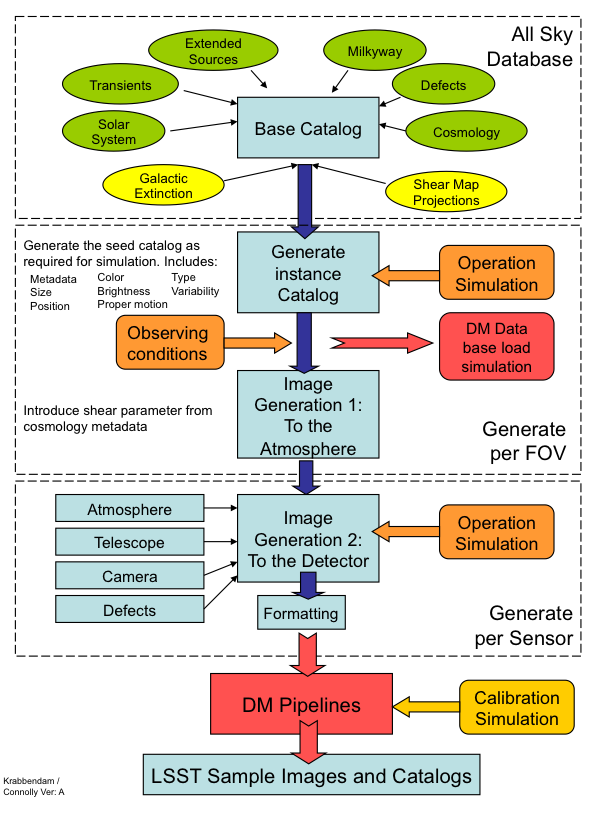
\includegraphics[width=6in]{validation_figures/flow.png}}
%
% If no graphics program available, insert a blank space i.e. use
%\picplace{5cm}{2cm} % Give the correct figure height and width in cm
%
\caption{The flow of information through the LSST simulation
  framework. Databases of astrophysical sources are populated with
  models of the cosmological distributions of galaxies, the
  distributions of stars within our Galaxy, and the populations of
  asteroids within our Solar System. Using historical records for the
  weather at Cerro Pachon and the observing cadences required by the
  science drivers for the LSST, sequences of simulated observations
  are generated by the Operations simulator. From these simulated
  pointings, catalogs and images of galaxies can be generated that
  match the expected properties of the LSST system. Comparing the
  catalogs derived by processing the LSST data with those used to
  generate the inputs we enable a full end-to-end test of the LSST
  system.}
\label{fig:flow}       % Give a unique label
\end{figure}


\subsection{Galaxies and Cosmology \label{sec:gal}}

The galaxy model is based on dark matter haloes from the Millennium
simulation \citep{springel05} with an assumed standard $\Lambda$-CDM
cosmology and a semi-analytic baryon model grafted upon the Millennium
results as described in \citet{springel05} and \citet{delucia}. This
semi-analytic model features radiative cooling, star formation, and
the dynamics of black holes, supernovae, and AGNs. It includes
novel features such as explicitly following dark matter haloes even
after accretion onto larger systems in order to follow the dynamics of
satellite galaxies for an extended period of time as well as 'radio
mode' feedback of AGNs. The model was adjusted to mimic the
luminosity, color, and morphology distributions of low redshift
galaxies \citep{delucia}. LSST cosmological catalogs were generated
by constructing a lightcone, covering redshifts 0$<$z$<$6, from 58
500h$^{-1}$Mpc simulation snapshots. This lightcone covers a 4.5x4.5
degree footprint on the sky and samples halo masses over the range
$2.5\times10^9$ to $10^{12}$ $M_\odot$. 

Dynamically tiling this footprint across the sky enables the
simulation of the full LSST footprint while keeping the underlying
data volume small (but at the expense of introducing periodicity in
the large scale structure).  For all sources, a spectral energy
distribution, is fit to the galaxy colors using Bruzual and Charlot
spectral synthesis models \citep{bruzual}. The
\citet{delucia} catalog includes BVRIK magnitudes and dust values for
the disk and bulge components of each galaxy as well as radii,
redshift, coordinates, stellar age, masses and metallicities. These
are also used in constraining the assignment of SEDs to each disk and bulge.
These fits are undertaken independently for the bulge and disk components and
include inclination dependent reddening. Morphologies are modeled using two
Sersic profiles and a single point source (for the AGN) with
bulge-to-disk ratios and disk scale lengths from \citet{delucia}.
 Half-light radii for bulges are estimated using the empirical
absolute-magnitude vs half-light radius relation given by 
\citet{gonzalez09}.  Comparisons between the redshift and
number-magnitude distributions of the simulated catalogs with those
derived from deep imaging and spectroscopic surveys showed that the de
Lucia models under-predict the density of sources at faint magnitudes
and high redshifts. To correct for these effects, sources are
``cloned'' in magnitude and redshift space until their densities
reflect the average observed properties (see
\ref{sec:galaxycounts}). 

AGNs are derived using the \citet{bongiorno12} luminosity function. The
B-band absolute magnitudes are converted to bolometric luminosities
using Eqn. 2 in \citet{hopkins07}. Empirical relations derived from the
SDSS enable computation of the colors and stellar mass of the AGNs
host galaxy from its luminosity. These parameters are used together
with the redshift values from the AGN catalog to match each AGN to a
galaxy in the galaxy catalog that best corresponds to the provided
values. In general, the AGNs match to galaxies having higher stellar
masses, approximately $10^{9}$ to $10^{11}$ $M_{\odot}$ which is
comparable to recent analysis of host galaxies done by \citet{xue11}. The
AGN SED is the \citet{vandenberk} mean AGN spectrum. 

\subsection{Galactic Structure \label{sec:stars}}

Stars are represented as point sourcesi and are drawn from the Galfast model of \citep{galfast}.  
Galfast generates stars according to
density laws  derived from fitting SDSS data
to a thick and thin disk along with a halo \citep{juric}. Using an 
input luminosity function measured from SDSS for each class of stars 
(main sequence, white dwarf, blue horizontal branch, etc.), Galfast samples stars in space and magnitude 
from a 4-dimensional probability density function
$\rho$(x,y,z,M). After this stage, using Fe/H and kinematics models
from \citet{ivezic08} and \citet{bond09} (also derived from SDSS data), 
the each star is assigned a metalicity, proper motion, and parallax.
Spectral energy distributions are fit to the predicted
colors using the models of \citet{kurucz93} for main sequence
stars and giants, \citet{bergeron95} for white dwarfs,
and a combination of spectral models and SDSS spectra for M, L, and T
dwarfs 
\citep[e.g.][]{cushing05,bochanski07,burrows06,pettersen89,kowalski10}. 
For Galactic reddening, a value of E(B-V) is assigned to each
star using the three-dimensional Galactic model of 
\citet{amores05}. For consistency with extragalactic observations the
dust model in the Milky Way is re-normalized to match the 
\citet{schlegel98} dust maps at a fiducial distance of 100 kpc.  Once the 
extinction and SED are assigned, observed magnitudes are calculated in
the SDSS and LSST photometric systems using fiducial system throughput curves.
Binary stars are included in the luminosity functions from which the
stellar colors are sampled but are assumed to be unresolved and
non-variable (except for a selection of eclipsing binarys described
later).

Stellar  populations included within the current implementation of the model are:
\begin{itemize}
\item Main Sequence: F,G,K,M,L,T
\item White Dwarf: H and He
\item Red Giant Branch
\item Blue Horizontal Branch
\item RR-lyrae
\item Cepheids
\end{itemize}

Approximately 10\% of the stellar sources are variable at a level detectable
by LSST.
Variability is modeled for sources within the base catalogs
by defining a light curve, its amplitude, a period, and a phase. For
queries that contain a time constraints the magnitude of the source is
adjusted based on the properties of the light curve (the current
implementation only allows for monochromatic variations in the
fluxes). Variables modeled range from cataclysmic variables, flaring
M-dwarfs, and micro-lensing events. For transient sources, the period
of the light curve is set to $>10$ years such that the sources will
not repeat within the period of the LSST observations.


\subsection{Solar System \label{sec:ssm}}

The solar system model is a realization of the \citet{grav11} model.  All
major groups are represented including: main belts, near earth
objects, trojans of the major planets, trans-neptunian objects, and
comets. There are approximately 11 million total objects with a vast
majority (about 9 million) being main belt asteroids. The populations
are complete down to apparent magnitudes of V=24.5.  Each object is
assigned a carbonaceous or stony composition spectrum derived from
extending the reflectance spectra from \citet{demeo} by linear
extrapolation from 4500$\AA$ to 3000$\AA$ and then multiplying by a
Kurucz model solar spectra. The choice of a C or S type spectra for an
object is assigned based upon a simple relation to the size of its
orbit that approximately matches SDSS asteroid observations. Each
object's brightness during a specific observation is calculated from
its location, phase, H\_V and g values. H\_V is the object's absolute
magnitude and corresponds to the brightness if it were observed at 1
AU from the sun and at zero phase angle. 
The $H_V$ distribution is modeled independently for each population (NEO,
TNO, main belt, etc.) as described in \S 3 of \citet{grav11}.
The g value
relates the change in brightness of an object with the change in phase
and is set at 0.15 for all objects across all bands which is a typical
value for asteroid phase curves.  A more accurate modeling of the asteroid
phase curves would require more realistic rotation and composition models which 
may be included in future work.
Adding the location of the Earth at the time of a particular observation, the
orbital ephemeris software oorb (\citet{granvik};{\tt http://code.google.com/p/oorb/}) calculates a V band apparent magnitude
which is then used with the object's assigned C or S type SED to
derive the corresponding LSST band observations.

\subsection{Query Framework}
The query framework is written in python and takes an object centric view of the 
data.  For each object type (galaxy, main sequence star, strong lens, etc.) a class
is defined that knows how to query for, format, and transform objects of that type.  
This approach provides an extensible framework as different components of the Universal model
are logically distinct and so can be separated into different tables in a database
or in different databases all together.

Many objects will be similar in terms of their properties and how they will be queried.
This allows a small number of base classes to be defined with most of the other object
classes as simplified subclasses of the the base.
Because of this a new object class is as simple as overriding the database connection string.

Extensibility of catalog types is handled by the InstanceCatalog class which defines how
the output from the object classes is formatted into catalogs.  Again, each catalog
type is a subclass of the base InstanceCatalog class, so extending to other catalog
types simply requires overriding the default formatter.  This also allows for custom headers
(like those needed for input to phosim) and custom output (e.g. binary, fits, or pickle).

\section{Validation of the Simulation Framework Requiremets}
The requirements for the catalog simulations (referred to as catsim) and described in sections
4.1 through 4.3 in the LSST simulations requirements document \citep{requirements}

\subsection{Requirement 1: The simulation framework shall be open source and the input data, configurations,
and software shall be accessible by the LSST project and science collaborations}
\begin{itemize}
\item {\bf Open source} -- All framework code is released under the GPLv3 license.
\item {\bf Accessible software and configuration} -- All framework code and configuration are 
stored in git repositories on the official LSST git server.
\begin{itemize}
\item {\tt https://dev.lsstcorp.org/cgit/LSST/sims/catalogs/generation.git/} -- Code to query
base catalogs.
\item {\tt https://dev.lsstcorp.org/cgit/LSST/sims/catalogs/measures.git/} -- Code to format
and manipulate catalogs produced by the generation packages.  This includes photometric, 
astrometric, and variability calculations.
\item {\tt https://dev.lsstcorp.org/cgit/LSST/sims/throughputs.git/} -- Repository
of system throughputs for the LSST reference design.
\end{itemize}
\item {\bf Accessible input data} -- All data are available via an MS SQL Database server
hosted and maintained by the University of Washington.
\end{itemize}

\subsection{Requirement 2: The simulation framework will be docuemented to a level that it can be
executed by external users}
In order to be useful to the community as a whole for trade studies and the evaluation of science 
capabilities, the simulation framework must be documented together with example applications.  

Documentation is available as web pages as well as self documenting docstrings within the code.  Documentation
is available on
at the following locations:
\begin{itemize}
\item catalog generation and measures -- {\tt http://www.astro.washington.edu/users/krughoff/documentation/}
\item base catalog schema and description -- {\tt https://dev.lsstcorp.org/trac/wiki/IS\_Catsim\_Database\_Documentation}
\end{itemize}

We have provided installation and example usage instructions for the catalog 
aspects of the framework at the links above.  
It has been installed and used at several locations 
including: SLAC, UC Irvine, Amazon EC2.

\subsection{Requirement 3: The interfaces between the components of the simulation framework shall be defined 
and documented}
The interfaces are:
\begin{itemize}
\item OpSim to CatSim -- This is documented and maintained by the OpSim team 
({\tt https://lsstcorp.org/sites/default/files/SSTARUserGuide.pdf}; accessed 07/29/2013)
\item CatSim to PhoSim -- This is documented and maintained by the PhoSim team and can be found in the document
{\bf XXX where is this}
\end{itemize}

\subsection{Requirement 4: The provenance within the data products shall be sufficient to rerun a simulation in a 
deteministic manner}
\begin{itemize}
\item OpSim -- Each run of the operations simulator is given unique identifier.  
The OpSim identifier provides a unique table naming convention in the OpSim database and is used by the catsim
query framework to select the observing conditions given a pointing and an OpSim run.
\item CatSim -- The base catalog data is stored on disk and is immutable. The base information
going into any given run is therefore the same.  Since the galaxies are tiled across the sky, the identifier returned
by the query framework is a combination of the tile number and the identifier from the base catalog ensuring that
all galaxies have a unique id and that that id is the same even if the observation parameters (e.g. boresite) are 
not the same from query to query.  The place where non-deterinism may enter is through the variability of the astrophysical
sources.
To enable a deterministic light curve (i.e. queries with a sequence of times) and account for the phase
an initial time, $T_o$, is defined.
Stochastic variability (e.g. damped random walk of AGN) that uses a random number generator is seeded by the same number for all identical runs.
\item PhoSim -- Input to the photon simulator includes a seed for the random number generator.  Since parallelism for
the photon simulator is on the chip level, the order of draws from the random number generator for each chip is the same.
\end{itemize}

\subsection{Requirement 5: The simulation framework shall be capable of running on individual workstations 
and high performance compute clusters}
CatSim runs naturally as a single core process since the problem is parallelized on a pointing by pointing basis.
To parallelize CatSim to larger systems many processes are run in a pleasingly parallel mode with each process running
a single pointing.  This approach marries nicely with schedulers like Portable Batch System ({\tt http://www.pbsworks.com/}, for example) 
and condor \citep{condor}.  
The limitation on the level of parallelism 
is the database I/O.  The current hardware (10 core, ??? GB, 40TB raid) has shown to be suitable up to 70 concurrent processes, 
resulting in ~200 pointings/day (~20\% real time).  The throughput can be improved with multiple servers or upgraded hardware.

\section{Validation of the Requirements on the Catalog Simulations}
The simulations catalogs in combination with tools for applying astrometric effects and a 
framework for generating observed catalogs provide all the requisite tools for conducting a 
wide range of analysis activities.
\begin{itemize}
\item For example, ealized positions of solar system objects can be used to test moving object detection algorithms.
\item Source catalogs can be used to test database and algorithm scaling.
\item Inputs generated for phosim using OpSim observing parameters enable large scale image simulation
for sensitivity analysis and algorithm development.
\item Realistic base catalogs allow science collaborations to inject specialized objects for specific science
analysis.
\item Time domain catalogs of variable objects allow testing of lightcurve recovery and characterization.
\end{itemize}

All of the examples above require a set of base catalogs that meet the project needs.  Where extensions to the types and
properties of sources are required (e.g.by the LSST science community), support for extensions fo the query 
framework is required.  

\subsection{Requirement 1: The LSST catalogs simulations shall contain representations of point,
extended, moving, and variable sources}

\subsubsection{Point, Extended and Moving Sources}
We have constructed a database to hold information about the sources required by the Universal model.
Each of these source types has their own schema (See sections \ref{sec:gal}, \ref{sec:stars}, and \ref{sec:ssm} for galaxies, stars, and solar system sources respectively).

The stellar schema is describe in {\tt http://ls.st/5jl}.  The database contains {\bf XXX} stars, covering the LSST footprint (Dec $< +30^o$)
and comprises tables for main sequence and red giant branch (??? stars), cepheids (), RR Lyrae (), blue horizontal branch (), and white dwarfs ().
For efficiency, large tables (e.g. the main sequence stars) are stored in zones each of {\bf XXX} deg wide.  All tables are indexed with a spherical
tree built using a hierarchical triangular mesh \citep[HTM][]{htm}. 

Galaxies are stored in a single table $4.5^o \times 4.5^o$ on a side with XXX galaxies. This single tile is then replicated across the sky to 
provide the spatial coverage needed to simulate the survey (see Figure \ref{fig:galcoverage}).  
Tiling of the galaxies is handled in the database using stored procedures (namely {\tt GalaxySearchSpecColsConstraint2013}).

The solar system model is the most complicated.  Since propogating orbits requires a numerical integration, it is very slow to do on 
11 million objects for every pointing.  In order to keep query times reasonable, at the very least, one needs a way to 
identify the obects that could possbily be in the frame.  Better yet would be a way to identify exactly (to the precision
required by LSST) where the objects that land in the aperture are located at a given time.  We have gone the second route.
The solution has two parts.  The first part is to preprocess the orbits by caching the orbit location every XXX seconds. 
These cached positions are then indexed using HTM to speed spatial lookup.
The second part is a stored procedure that uses the spatial index to produce a set of likely candidates and then applies
an interpolation algorithm to get the exact position of each candidate.

For all sources the generation of magnitudes and color, and the application of time dependent astrometric corrections (e.g. 
precession, parallax, proper motion) are calculated by python subclasses of the InstanceCatalog object.

\subsubsection{Variable Sources}
The framework is able to support several types of variability: periodic, stochastic, repeating.
The variability models used in the database include:.  
\begin{itemize}
\item M-dwarf flares -- full sky
\item AGN/QSOs -- full sky
\item RRly -- full sky
\item Cepheids -- exemplar individuals
\item Eclipsing binaries -- exemplar individuals
\item Am CVn -- exemplar individuals
\item Micro lensing -- exemplar individuals
\end{itemize}
Each model is described by either a parametric model or an interpolated lookup table.  To date only mono-chromatic variability has been implemented.
See Figure \ref{fig:lcs} for some example lightcurves.

The variable sources are implemented as a python API used by the InstanceCatalog object to adjust the brightenss of the sources based on the observation time.
The API calls for a dictionary of parameters to be passed to the appropriate method for application at generation time.  The name of the variability method and
the parameters describing a particular object's variability are stored in the database with the rest of the object properties.

\subsection{Requirement 2: At high Galactic latitudes the average source densities of stars and galaxies
shall be within 18\% of the observed counts (to the 5$\sigma$ point source coadded depth of LSST)}
The motivation for this requirement is two fold.  There is a functional requirement that the distribution of sources is representative
to test database scaling and I/O sizing models.  

Stellar number densities at galactic latitudes closer than to the plane than $|b| < 30^o$ are difficult to model due to the rising density and resulting confusion and deblending issues.
For these reasons, the criterion for stellar number counts at low latitudes are relaxed to $\pm 30\%$. 
For stars where $|b| > 30^o$, the Galfast model has been vetted against the SDSS data.  For stars with $|b| < 30^o$, we quantify the uncertainty in the model by comparing two reference models for Galactic structure.
We compare the realization of the Galfast model to a realization of the \citet{besancon} model.

\subsubsection{Stars}
We take six representative fields at varying galactic latitude at two longitudinal values (one toward the bulge, $b=0$, and one away, $b=180$).  
We compare number 
counts of main sequence stars to the coadded limiting magnitude in i-band 
 from the Galfast model using the composite dust model
of \citet{amores05} normalized to \citet{schlegel98} to the \citet{besancon} model with their dust model.  Figure \ref{fig:scounts_0} shows 
the cumulative number counts as a function of magnitude for the Besan\c{c}on (dashed) and Galfast (solid) models 
for six values of galactic longitude toward the galactic bulge.  We are interested in the
fractional cumulative contribution.  In Figure \ref{fig:sratio_0} we plot the ratio of Besan\c{c}on counts to Galfast counts for the six test fields shown in Figure \ref{fig:sratio_0}.
The dashed lines are the $\pm30\%$ limits for the low latitude sizing model constraints and the dash-dot lines are the $\pm18\%$ limits for the high latitude limits.
Since the number counts are dominated by the faint end, it's most important where the lines end up at faint magnitudes for sizing considerations 
(the coadded depth for the i-band is 26.8).  
Nominal single epoch depth for i-band is 24.0.  

In the case directed toward the galactic bulge, all fields meet the requirements at the coadded depth except
for $b=-10$.  At the nominal single epoch depth, the $b=-10$ case fails and the $b=-30$ case misses the $\pm18\%$
requirement, but makes the $\pm30\%$ requirement.

For the high latitude fields away from the galactic bulge, the deviation from the Besan\c{c}on model is within 
the stated requirement.  The $b=-10$ case, the number counts from Galfast significantly under predict relative to 
the Besan\c{c}on model.  The $b=-30$ case shows similar, though not as drastic, under prediction and misses the 
requirement for all but the faintest magnitudes and even then only meats the $\pm30\%$ requirement.

%We repeated this analysis using the GALFAST dust model and the results do not change significantly
\begin{figure}[H]
\centering
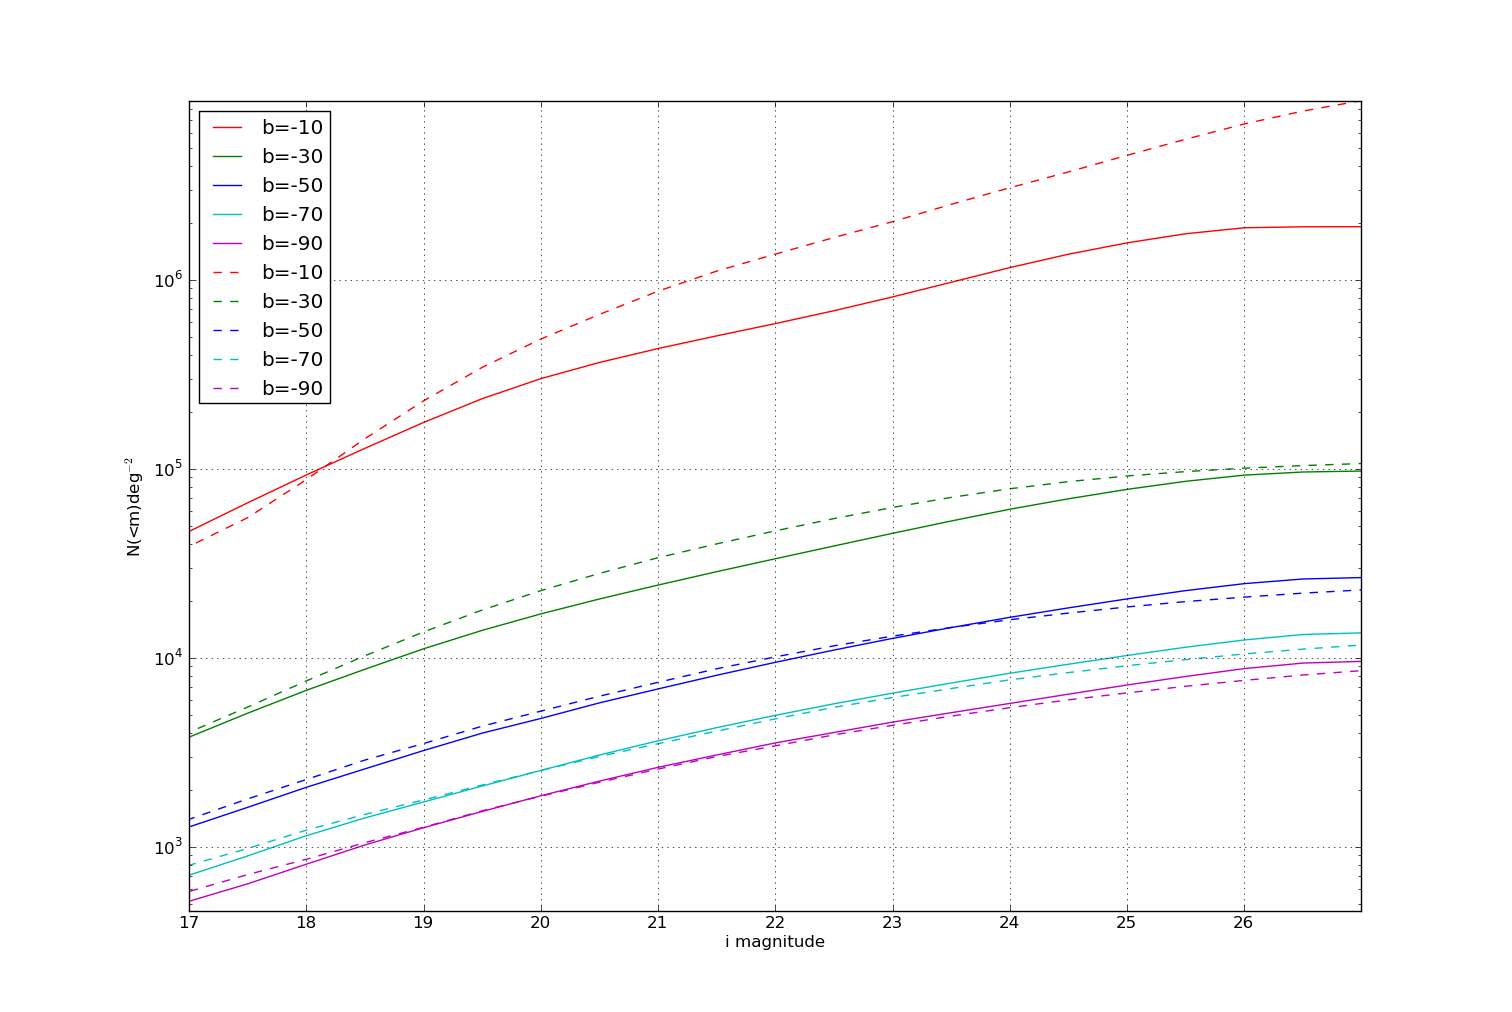
\includegraphics[width=5in]{validation_figures/cumulative_stars_0_besancon_dust.png}
\caption{Cumulative counts of stars from the Besan\c{c}on (dashed) and Galfast (solid) models for 5 representative fields toward the Galactic bulge (l=0$^o$) \label{fig:scounts_0}}
\end{figure}
\begin{figure}[H]
\centering
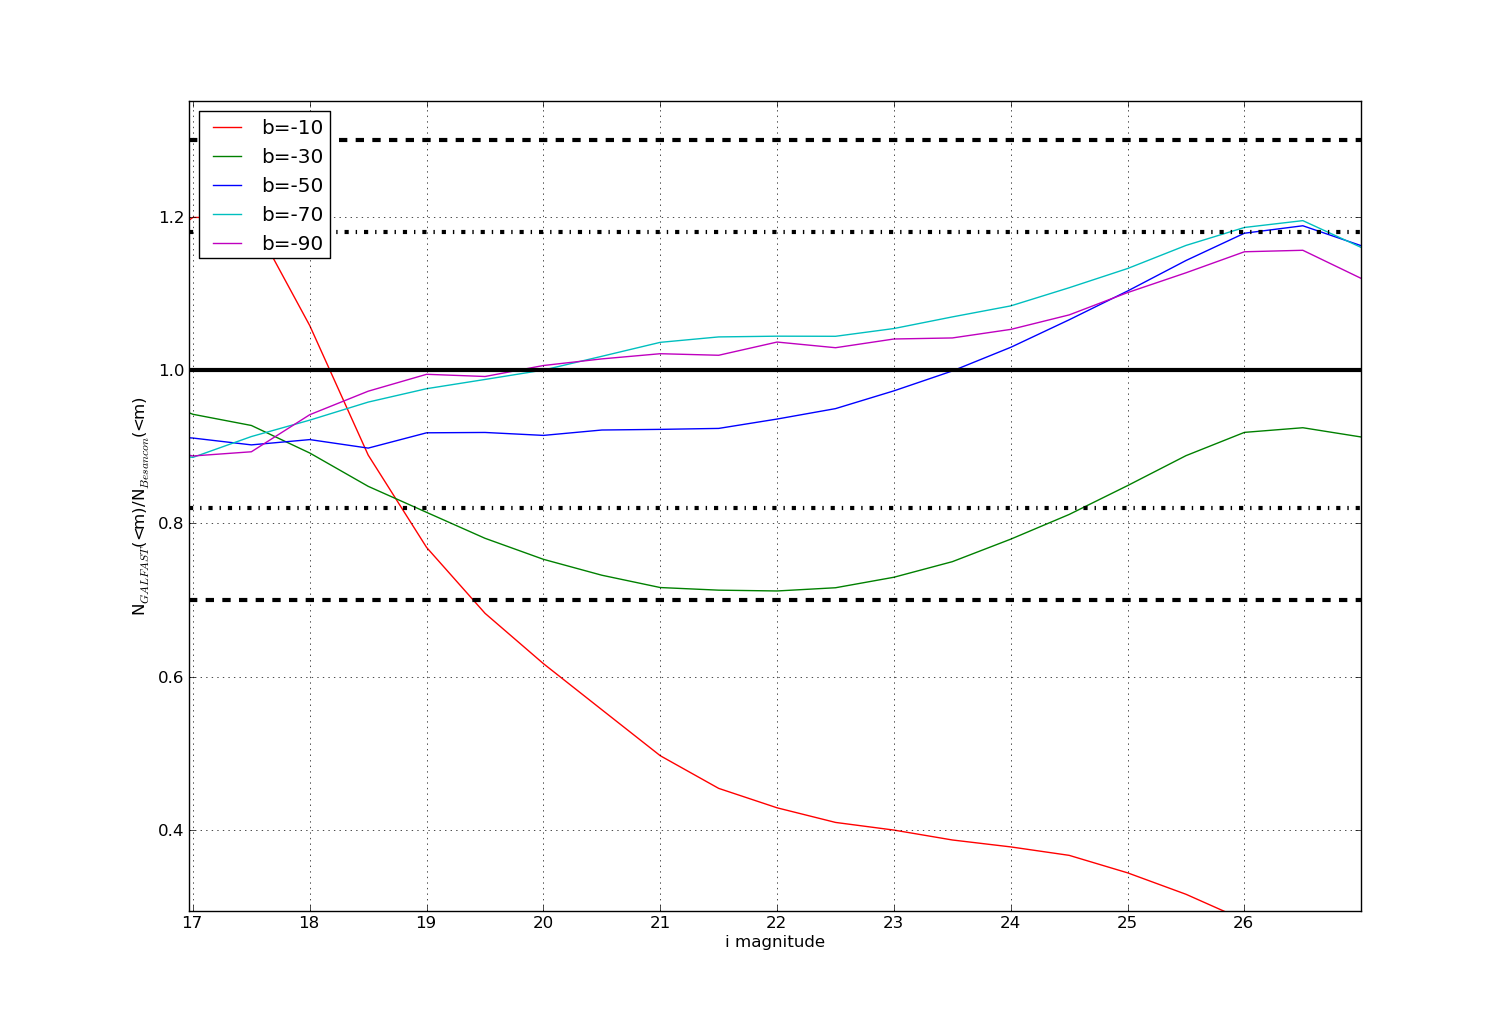
\includegraphics[width=5in]{validation_figures/cumulative_ratio_stars_0_besancon_dust.png}
\caption{Cumulative ratio of counts of stars from the Besan\c{c}on and Galfast models for 5 representative fields toward the Galactic bulge (l=0$^o$) \label{fig:sratio_0}}
\end{figure}
\begin{figure}[H]
\centering
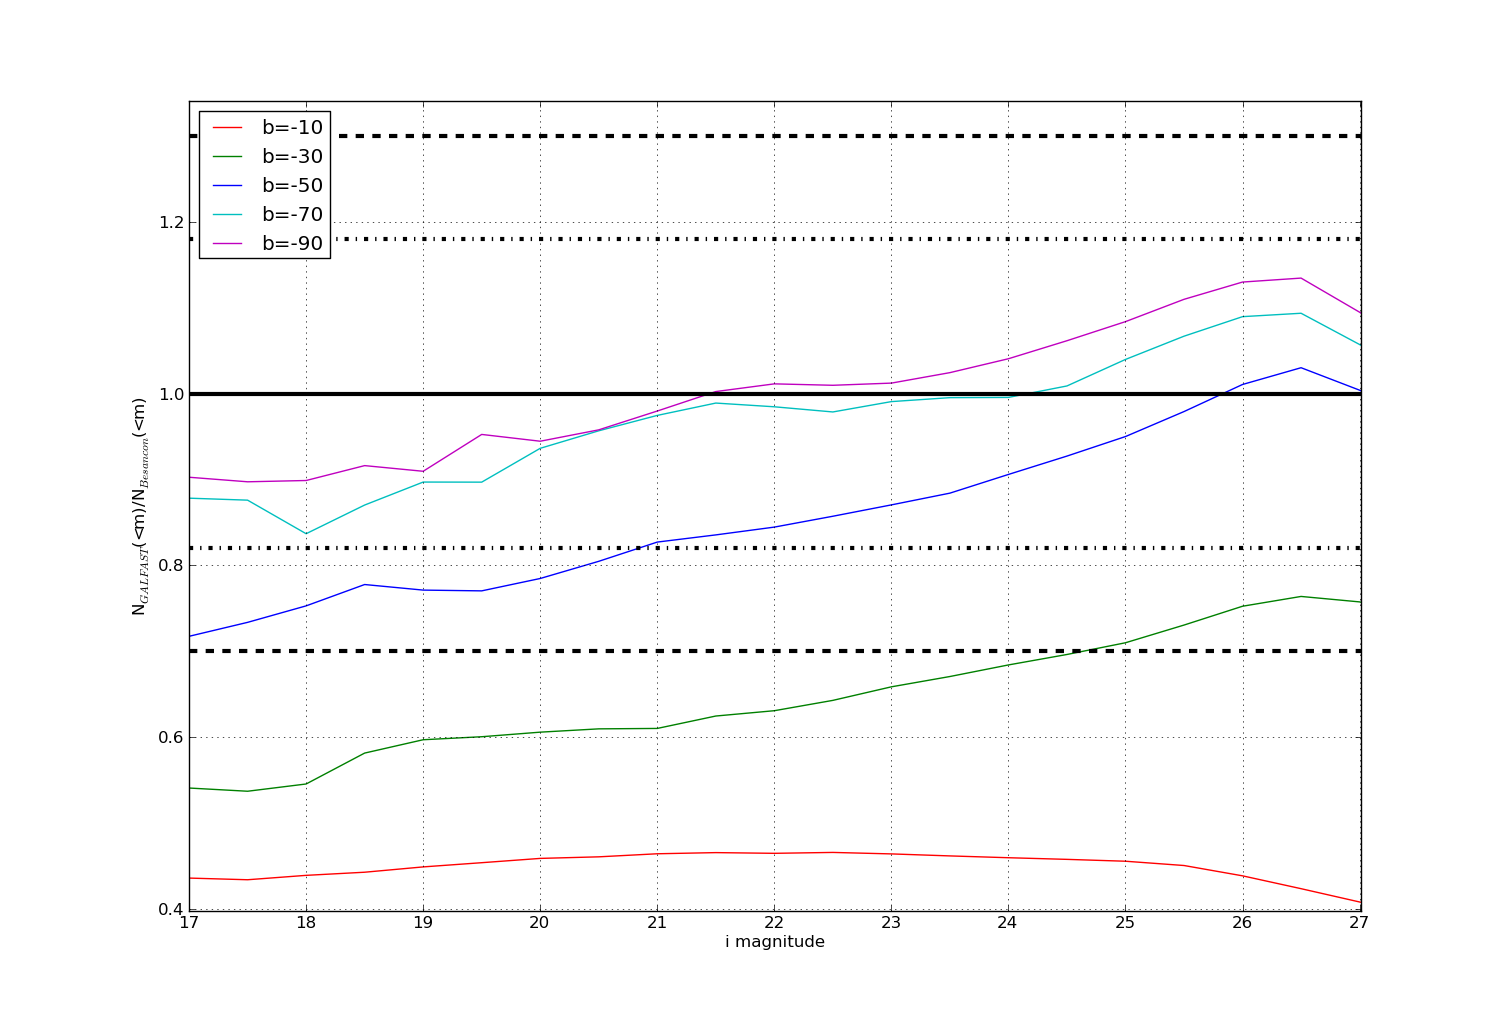
\includegraphics[width=5in]{validation_figures/cumulative_ratio_stars_180_besancon_dust.png}
\caption{Cumulative ratio of counts of stars from the Besan\c{c}on and Galfast models for 5 representative fields away from the Galactic bulge (l=180$^o$) \label{fig:sratio_180}}
\end{figure}

\subsubsection{Galaxies \label{sec:galaxycounts}}
We compare the galaxy counts to those provided by Metcalfe et al. (see {\tt http://star-www.dur.ac.uk/~nm/pubhtml/counts/counts.html}; 
accessed 07/29/2013).  We have taken their compilations from:
{\tt http://star-www.dur.ac.uk/~nm/pubhtml/counts/idata.txt} accessed on 06/01/2013.  
We include those data points with error bars.  
Using these counts
we noticed that the numbers of galaxies were under predicting at faint magnitudes.  

The result of the nubmer counts as a function of magnitude (after the cloning correction see \S \ref{sec:gal}) are shown in Figure \ref{fig:gcounts}.  
We have chosen the i-band data for comparison to 
minimize the effects of dust extinction which are somewhat uncertain in the Durham compilations.  A single transform from Kron-Cousins to AB of I$_{kc}$ = i$_{AB}$ - 0.5 was applied to
all compliation data.  For comparison with requirements on the sizing model stated in the requirements document, we also plot the cumulative ratio of the best fit polynomial
to the Durham data to the counts from the base catalog.  The requirement is $\pm18\%$ to the coadded i-band depth of 26.8.  We see that the base catalog
underpredicts at the faintest magnitudes, but meets this requirement (Figure \ref{fig:gratio}).

\begin{figure}[H]
\centering
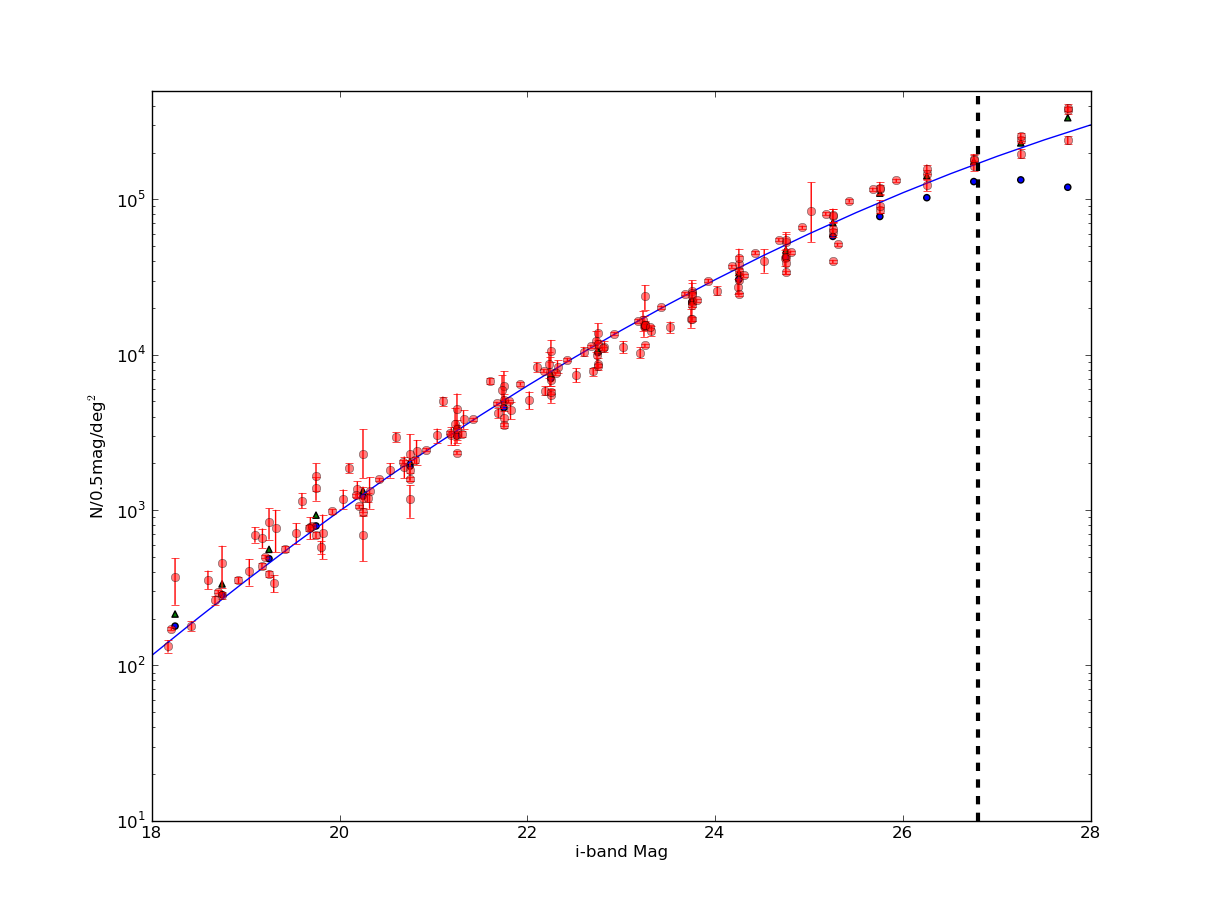
\includegraphics[width=5in]{validation_figures/Ngals-i.png}
\caption{Durham counts (symbols) compared to the counts from the base catalog \label{fig:gcounts}}
\end{figure}
\begin{figure}[H]
\centering
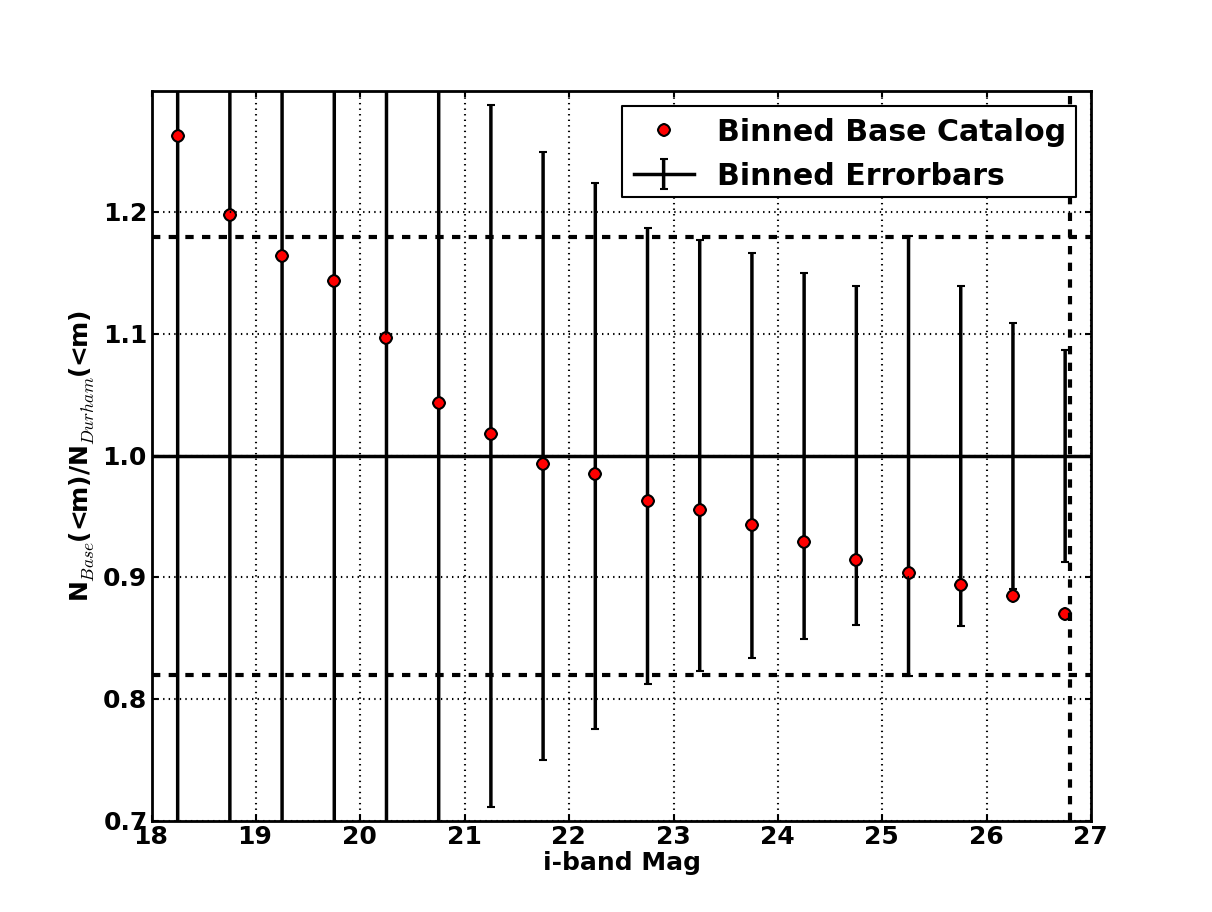
\includegraphics[width=5in]{validation_figures/CumulativeFraction_i.png}
\caption{Durham counts divided by the counts from the base catalog.  Error bars are from adding the error bars from the data points in quadrature. \label{fig:gratio}}
\end{figure}

\subsubsection{Ramifications of missing requirements}
At low galactic latitiudes the models for the stars are uncertain at a level greater than the requirements (i.e the discrepancy between Galfast and Besancon is > {\bf XX}\%).  This has the potential to impact the sizing and compute models for the LSST.

The validity of the Besan\c{c}on as ground truth in the plane of the galaxy is not obvious.  In fact, SDSS and galfast star counts agree surprisingly well at low galactic latitudes (private communication with M. Juri\'{c}). 
However, the completeness of SDSS deep in the plane has also not been quantified.  Certainly in the densest regions
of the plane there is significant loss of stars due to blending.  Further, since the Besan\c{c}on models are drawn
from distributions with binary corrections applied and the Galfast model does not produce unresolved binary systems
as multiple objects in the catalogs, the Galfast models will underpredict relative to the Besan\c{c}on by 
approximately the unresolved binary fraction.  These questions will be resolved through an ongoing comparison to observations
from other surveys (e.g. Pan-STARRS).

\subsection{Requirement 3: Size, ellipticity and redshift distributions of galaxies shall be representative of those observed by extant
telescopes and, for a fiducial image quality of 0.7 arcsec, deviations from the observed distributions shall
contribute $< 20\%$ of the observed effective density of galaxies, $n_{eff}$, used in the weak lensing samples (with a fiducial value of
$n_{eff} = 34$ galaxies per arcmin$^2$}
\subsubsection{Motivation}
The measurement of weak lensing is dependent 
on $n_{eff}$ which is the effective density of galaxies on the sky that can be used to measure weak lensing.  
The value of $n_{eff}$ depends on the inherent shape noise, the signal-to-noise distribution and the size distribution relative to the PSF.



\subsubsection{Measuring $n_{eff}$}
We use the framework described in \citet{chang} to calculate $n_{eff}$ for the distributions in the 
base galaxy catalog.  In summary, we use Equation 9 to calculate $n_{eff}$:
\begin{equation}
n_{eff} = \frac{1}{\Omega}\sum^N_i\frac{\sigma^2_{SN}}{\sigma^2_{SN}+\sigma^2_{m,i}}
\end{equation}
where $\sigma_{SN}$ is the intrinsic shape noise and $\sigma_{m,i}$ is the shape measurement noise for the i$^{th}$ galaxy.

The shape noise is derived from the ellipticity distribution.  For the distribution used in \citet{chang} $\sigma_{SN} = 0.26$.
The measurement noise can be approximated using Equation 13:
\begin{equation}
\sigma_m(\nu,R) = \frac{a}{\nu}\left[1+\left(\frac{b}{R}\right)^c\right]
\end{equation}
Where $\nu$ is the signal-to-noise ratio of the measurement, $R=\frac{r_{gal}^2}{r_{PSF}^2}$ is the size of the galaxy relative to
the point spread function.  We adopt values from \citet{chang} of (a,b,c) = (1.58,5.03,0.39), and assume a fiducial
PSF size of 0.7 arcsec. We use an estimate for the limiting magnitude of the coadded images
of 26.7.  This takes into account the fact that the measurements are on extended sources as well as the fact that the SRD value 
of 27.5 in r is for dark sky observations at zenith.   The galaxy sample is the ``Gold Sample'' of galaxies with $i < 25.3$.
For each galaxy, $r_{gal}$ can be calculate from the flux ratio of the bulge and disk components as well as the effective half light 
radii of each component (see Appendix B in \citet{chang} for a derivation of this calculation).

Using this framework, we test the sensitivity of the measured $n_{eff}$ on the ellipticity and size distributions.  For all calculations that follow we 
use the k=1 criterion of \citet{chang} meaning that galaxies with $\sigma_m < \sigma_{SN}$ are culled from the sample.

The shape noise distribution was well measured by the COSMOS project \citep{cosmos} and, to first order, is just the variance in the measured 
ellipticity distribution.  The $n_{eff}$ depends strongly on the apparent magnitude because of the steepness of the galaxy number
counts, but because of the dependence on signal to noise it has
has a very sharp cutoff at around i=24.5 (see Figure \ref{fig:neffvm}).  Galaxy redshift distributions must
agree with observations to this limiting magnitude to assure accurate signal to noise distributions.  Finally, the size distribution
of the combined two component galaxy model must match measured distributions closely in order to reproduce predicted
values of $n_{eff}$ from measured distributions.  We measure the distribution from the base catalogs and show that it is well
within the envelope necessary to reproduce realistic values of $n_{eff}$.

The ellipticity distribution is measured from the base catalog by sampling the appropriate composite Sersi{\'c} (bulge and disk together) using the
elipsoid parameters and flux ratio for each galaxy.  The moments are measured and ellipticities are calculated using the definitions in \citet{chang}.
\begin{equation}
\epsilon_1 = \frac{I_{11}-I_{22}}{I_{11}+I_{22}+2\sqrt{I_{11}I_{22} - I^{2}_{12}}}\\
\epsilon_2 = \frac{2I_{12}}{I_{11}+I_{22}+2\sqrt{I_{11}I_{22} - I^{2}_{12}}}
\end{equation}
We measure the same value of shape noise as reported by \citet{chang}, $\sigma_{SN} = 0.26$.  The shape appears to be slightly different than
that of the COSMOS sample, but we have not investigated the effect of distribution shape on the measured value of $n_{eff}$ (see Figure \ref{fig:ellip1} 
and Figure \ref{fig:ellip2}).  
Slight variations in
ellipticity distribution shape will not impact the measured value of $n_{eff}$ enough for the catalog to miss the requirement.  Figures \ref{fig:ellip_errbig}
and \ref{fig:ellip_errsmall} show the measured ellipticity distribution from the base catalog scaled such that the $n_{eff}$ requirement would be missed on the high side 
and on the low side respectively.
\begin{figure}[H]
\centering
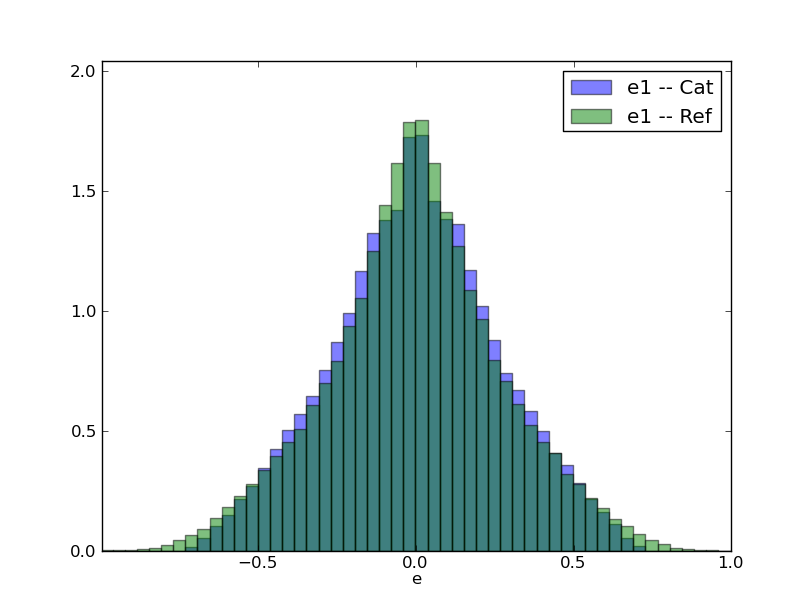
\includegraphics[width=5in]{validation_figures/e1_hist.png}
\caption{Histogram of e1 values for the base catalog and COSMOS sample.  These distributions are for objects with $20.0 < i < 24.5$ to match
the cut made in \citet{chang}.\label{fig:ellip1}}
\end{figure}
\begin{figure}[H]
\centering
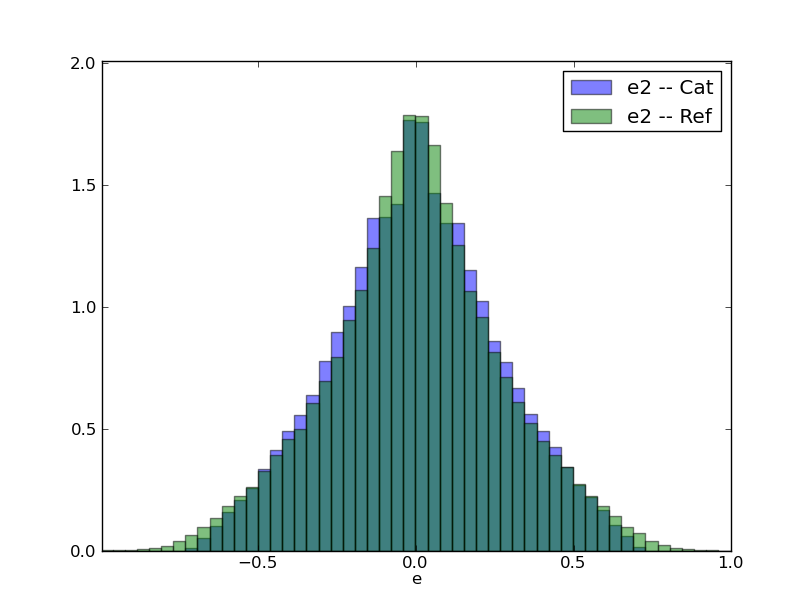
\includegraphics[width=5in]{validation_figures/e2_hist.png}
\caption{Same as Figure \ref{fig:ellip1} but for e2.\label{fig:ellip2}}
\end{figure}

\begin{figure}[H]
\centering
  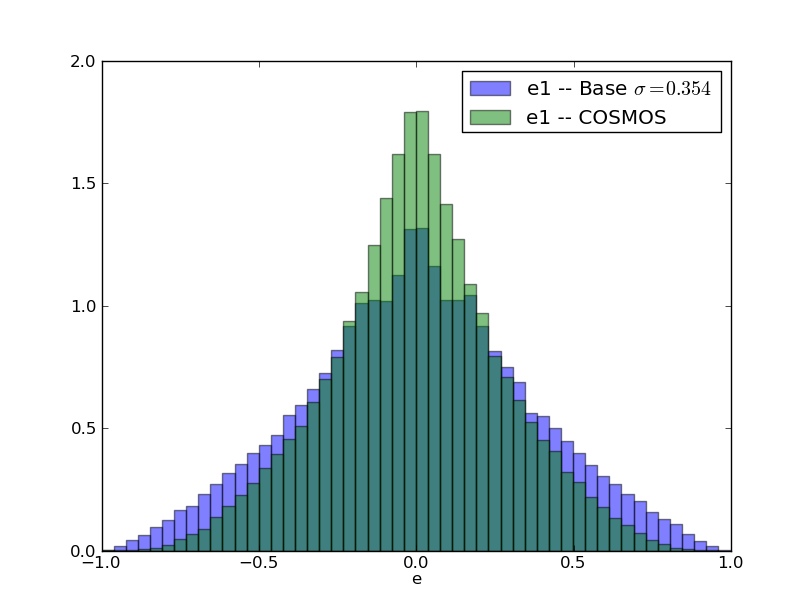
\includegraphics[width=5in]{validation_figures/e1_hist_s_354.png}
\caption{The base catalog distribution with the width scaled such that the requirement is just missed by predicting an $n_{eff}$ value that is too large.\label{fig:ellip_errbig}}
\end{figure}
\begin{figure}[H]
\centering
  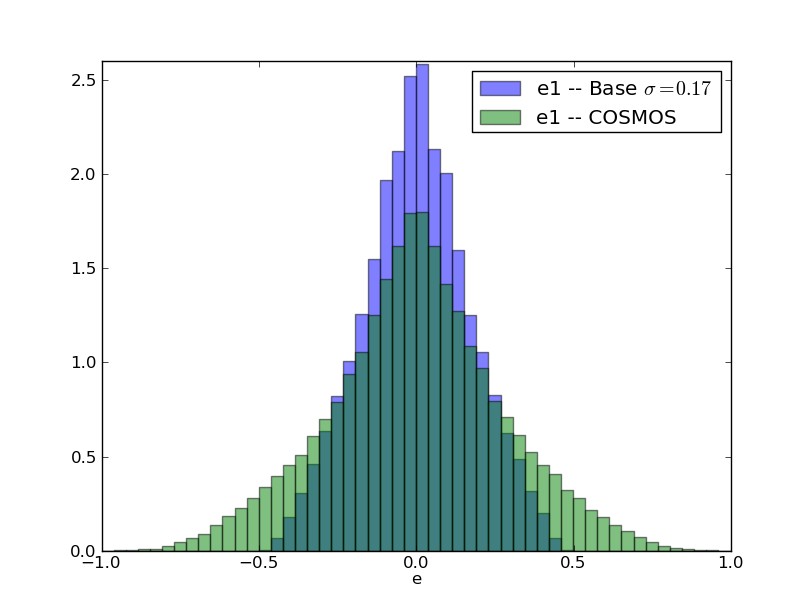
\includegraphics[width=5in]{validation_figures/e1_hist_s_17.png}
\caption{The base catalog distribution with the width scaled such that the requirement is just missed by predicting an $n_{eff}$ value that is too small.\label{fig:ellip_errbig}}
\end{figure}

For completeness, we show the redshift distributions for 1 magnitude bins from $i=18$ to $i=24$.  See Figure \ref{fig:nofz18_24}.  As shown in \ref{fig:neffvm}
galaxies with $i > 25$ do not contribute significantly to $n_{eff}$. 
\begin{figure}[H]
\centering
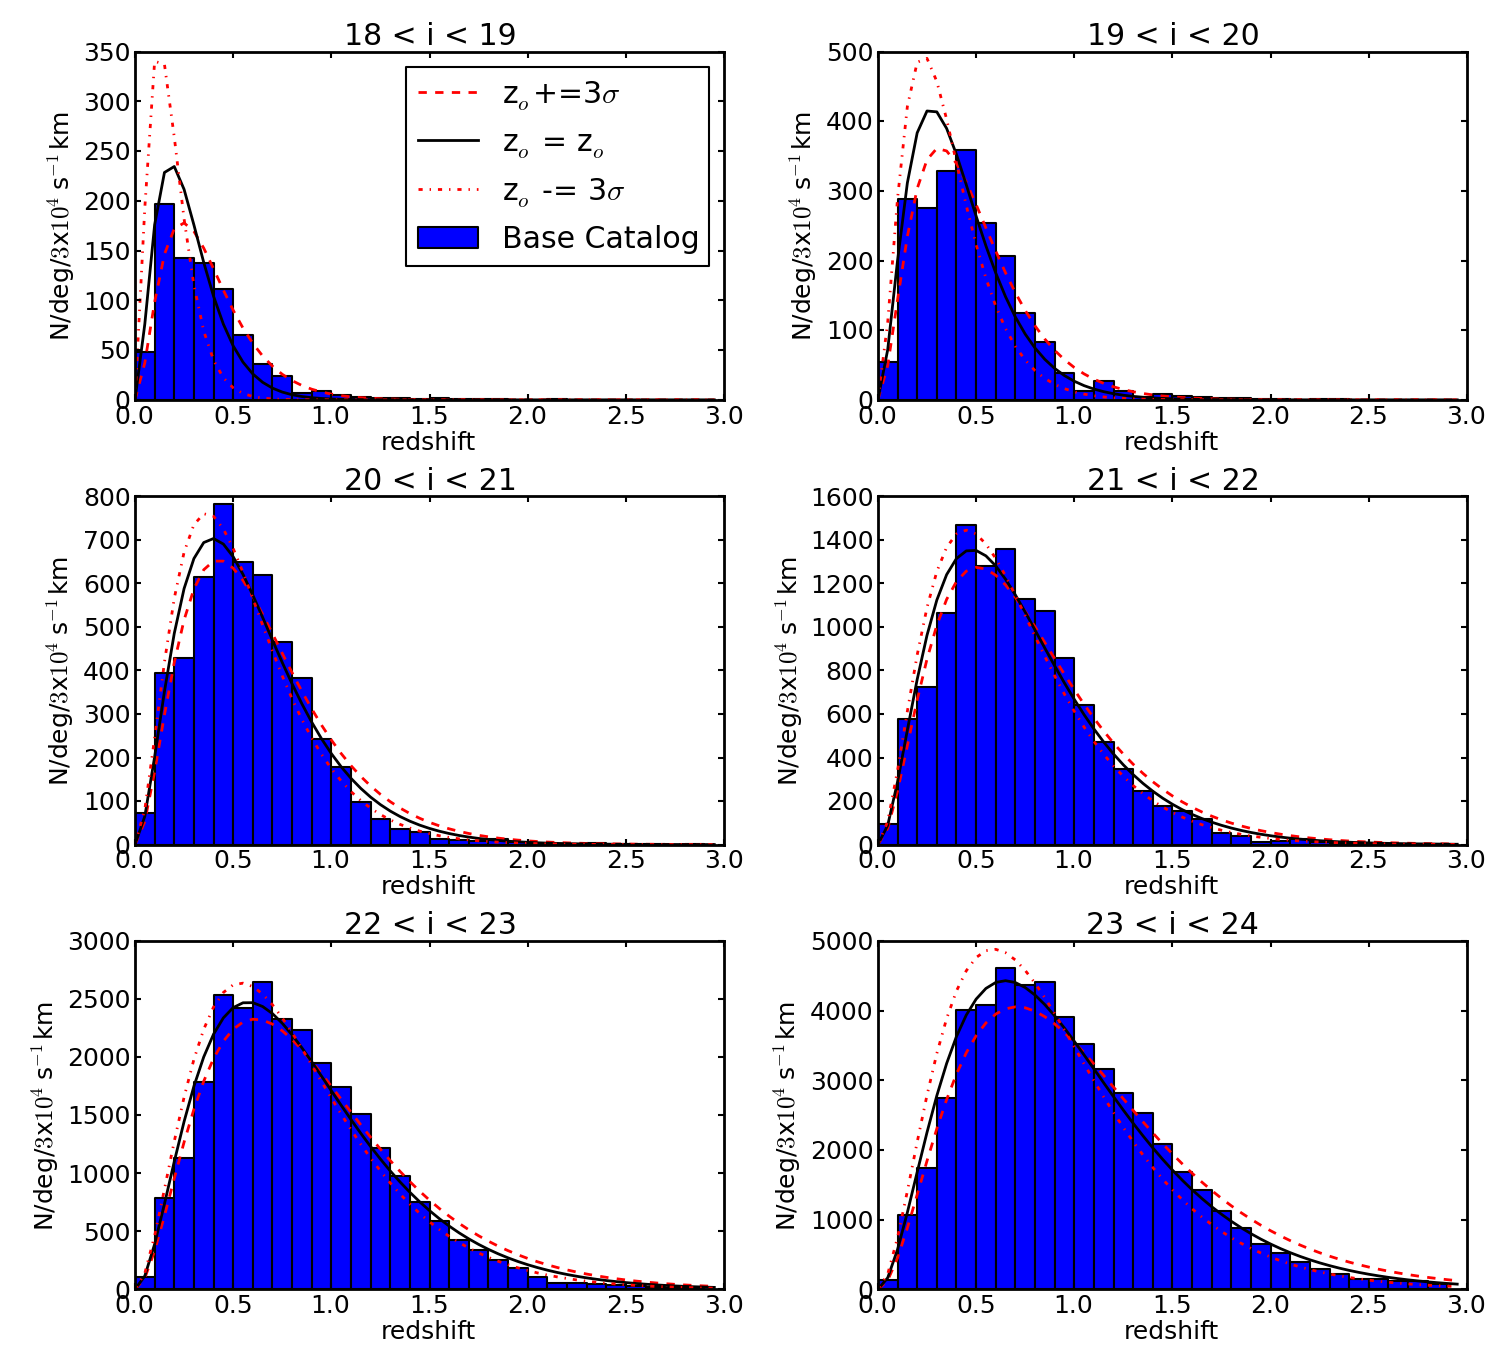
\includegraphics[width=5in]{validation_figures/Nofz_18_24.png}
\caption{The blue histogram in each panel is the measured N(z) for 1 magnitude bins from $18<i<24$.  Overplotted is the empirical distribution from \citet{coil04} normalized to the area of the measured distribution.  The dashed and dotted red lines show what happens if the governing parameter for the \citet{coil04} distribution, $z_o$, is over
or under predicted by $3\sigma$ respectively.\label{fig:nofz18_24}}
\end{figure}
%\begin{figure}
%\centering
%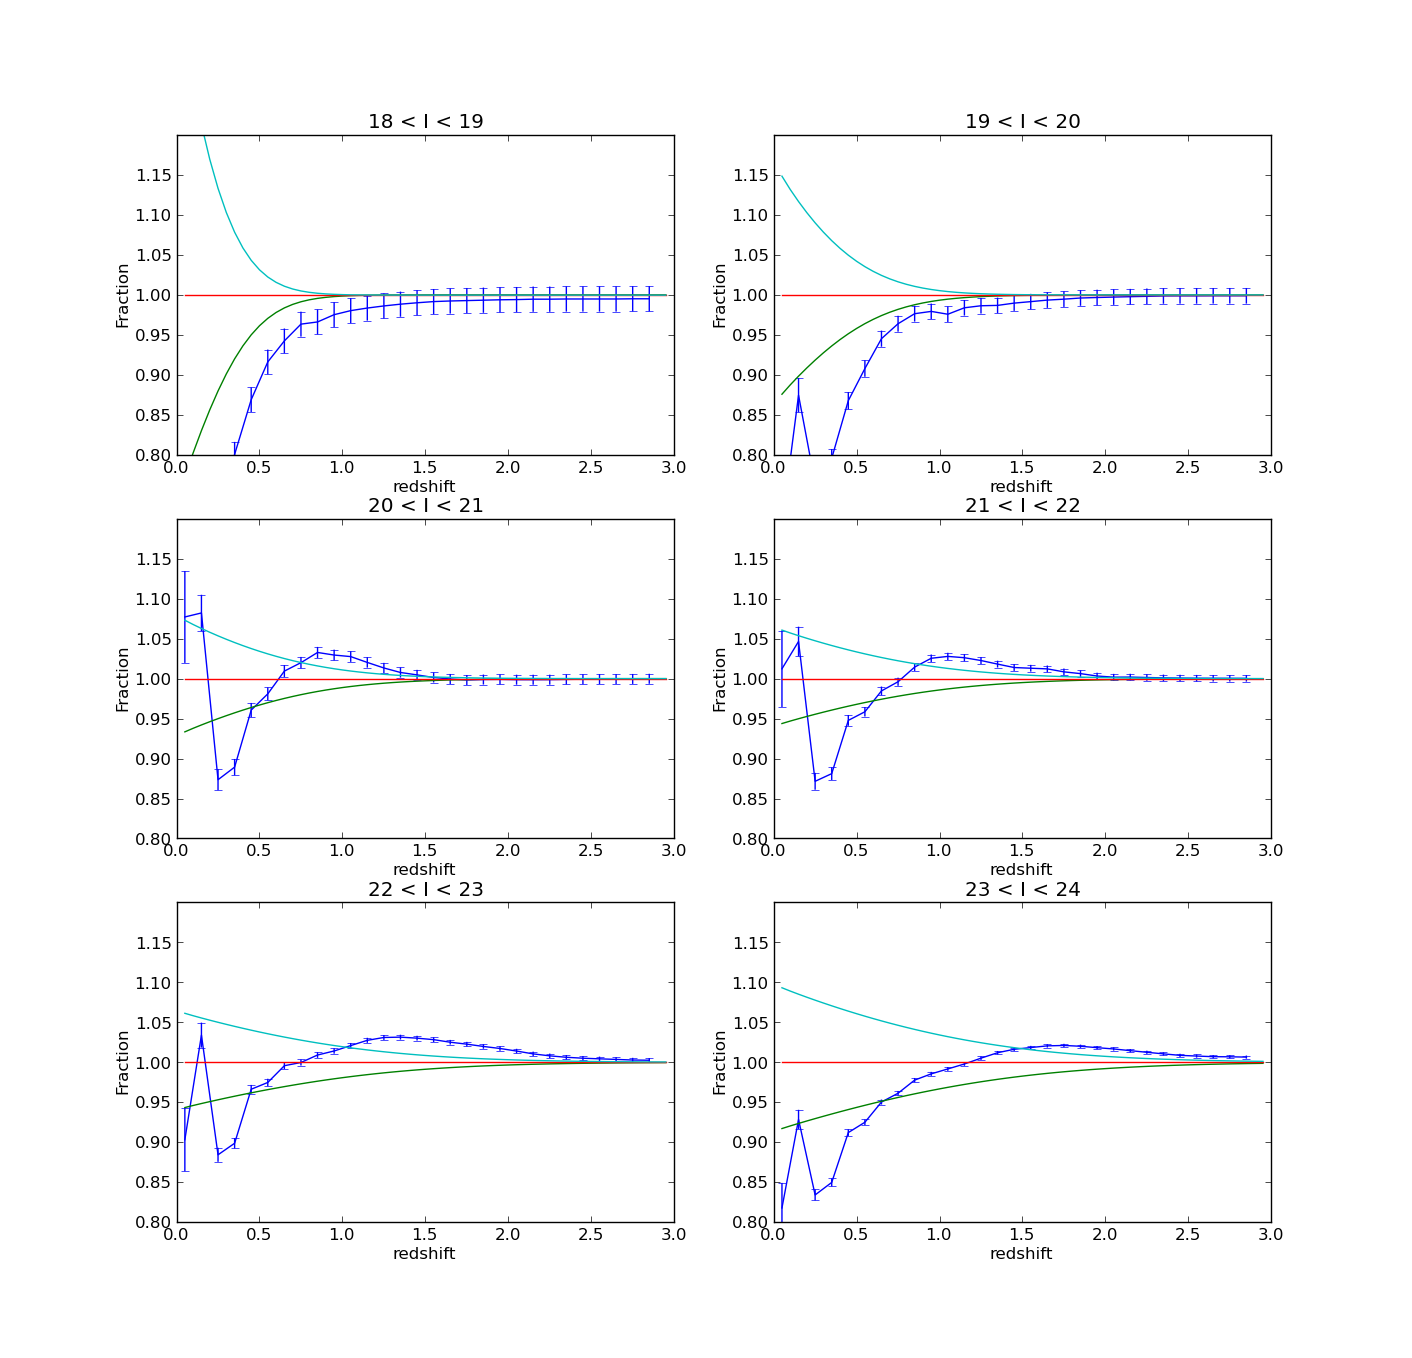
\includegraphics[width=5in]{validation_figures/Nofz_CumulativeFraction_18_24.png}
%\caption{N(z) for 18 to 24 with distribution from \cite{coil}\label{fig:nofz18_24_ratio}}
%\end{figure}
%\begin{figure}
%\centering
%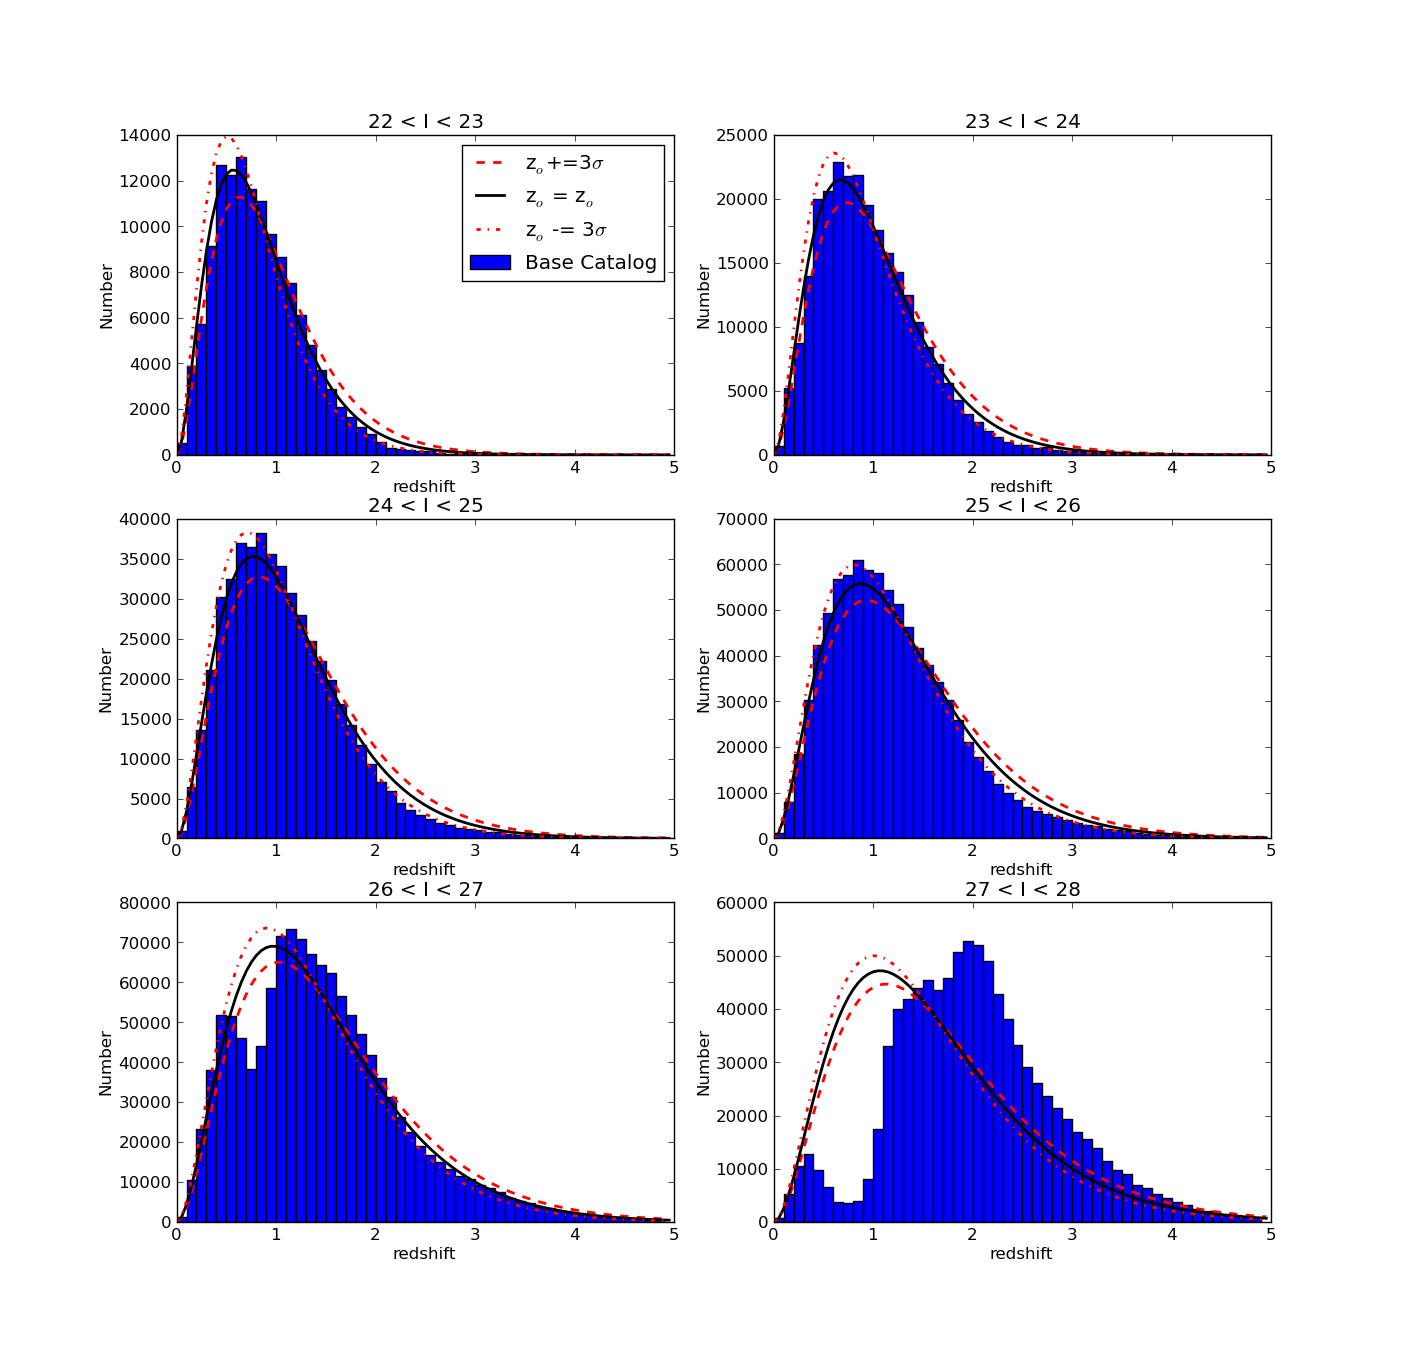
\includegraphics[width=5in]{validation_figures/Nofz_coil_22_28.png}
%\caption{N(z) for 22 to 28 with distribution from \cite{coil}\label{fig:nofz22_28}}
%\end{figure}
%\begin{figure}
%\centering
%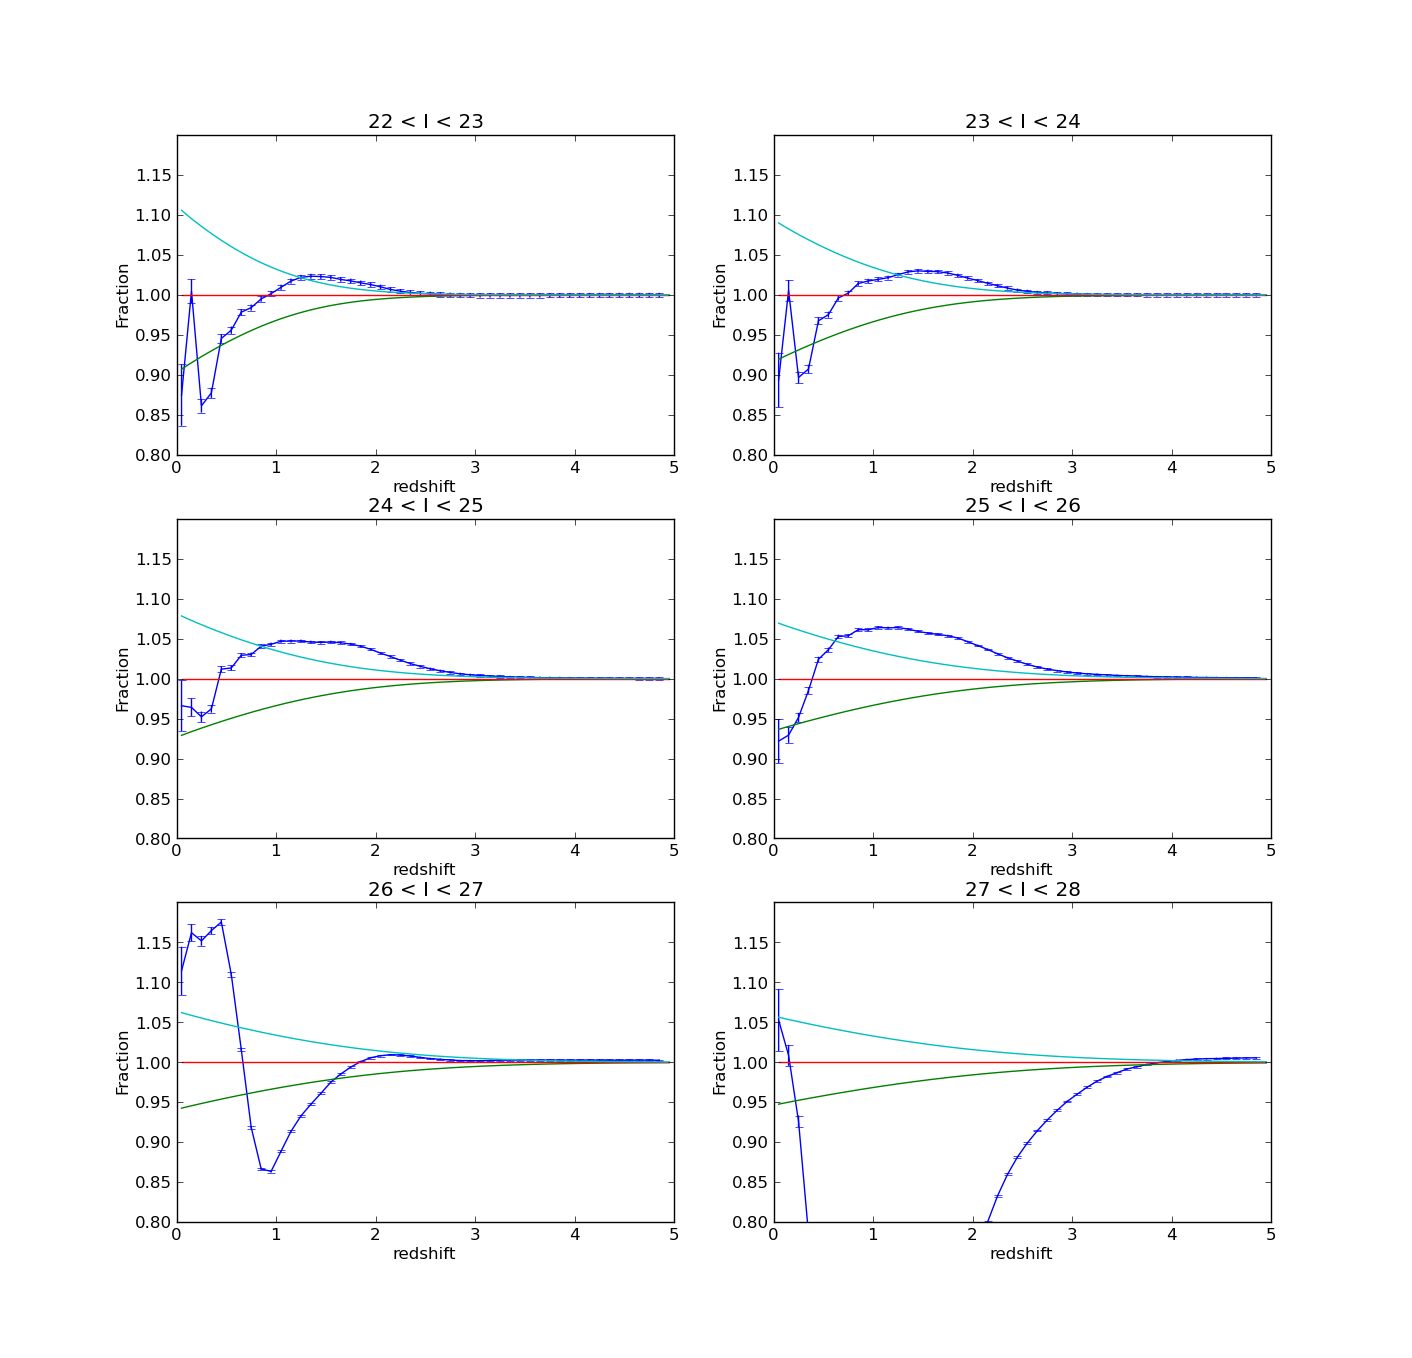
\includegraphics[width=5in]{validation_figures/Nofz_CumulativeFraction_22_28.png}
%\caption{N(z) for 22 to 28 with distribution from \cite{coil}\label{fig:nofz22_28_ratio}}
%\end{figure}
\begin{figure}[H]
\centering
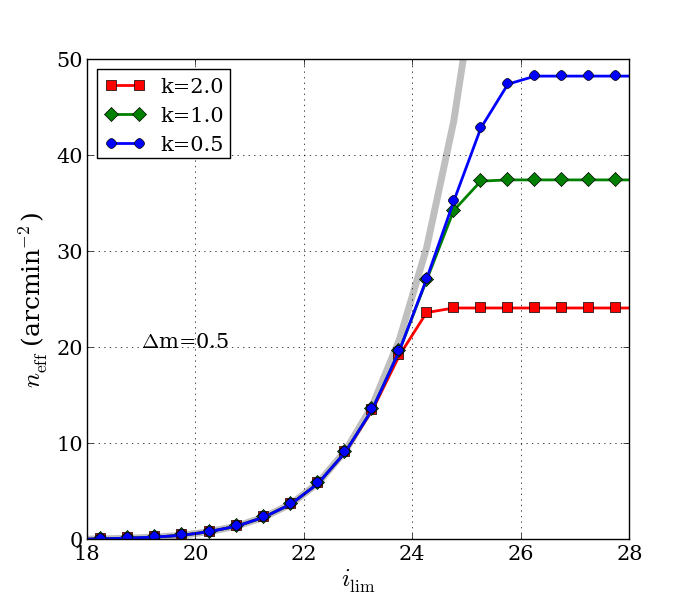
\includegraphics[width=5in]{validation_figures/neff_m_ir.png}
\caption{This shows $n_{eff}$ as a function of i-band limiting magnitude.  Even though the the density of galaxies is going up steeply, the 
size of the galaxies relative to the PSF is falling off quickly enough that galaxies fainter the $i=25$ don't contribute much to $n_{eff}$.\label{fig:neffvm}}
\end{figure}

{\bf XXX read to here}

\subsubsection{Galaxy radius measurements}
There are many definitions of galaxy size: half light radius, first moment radius, second moment radius, Petrosian radius, Kron radius, etc.
oOur comparison data set is that from the COSMO ACS catalog \citep{cosmos} because of the size ($~2deg^2$), depth ($~26$ in i), and
quality (space based).  

The COSMOS catalog reports the second moments and the 
half light radius, so either the second moment radius or half light radius could be used for comparison.  One concern is that the measurements
on the base catalog are effectively infinite signal to noise, whereas the measurements from COSMOS are not.  
We consider the impact of the S/N on the derived quantitiesin order to define the appropriate measure to use for comparison.
To measure the sensitivity of the half light radius and second moment radius to the effects of S/N we 
sample from truncated Sersi{\'c}
profiles for each galaxy.  Measurement on a truncated profile is an estimate of the same measurement made on a noisy profile that drops below
the noise at the truncation radius as the noise should contribute to the moments symmetrically.
We truncate the profiles at several multiples of the half light radius, $R_{hl}$: $1.33R_{hl}, 1.78R_{hl}, 3.16R_{hl}, 10R_{hl}, $and$100R_{hl}$
We see this in the
half light radius distribution as well, but at a much lower level.  See Figure \ref{fig:mom_hist} and Figure \ref{fig:hl_hist}.  Figure
\ref{fig:mom_hl_line} shows that the half light distribution shape measurements are flat down to truncation at 3 half light radii, where 
the second moment radius distribution is not stable even going from 100 to 10 half light radii.  For these reasons, we choose to compare the half light 
radius distribution to the half light radius distribution from the COSMOS catalog.
\begin{figure}[H]
\centering
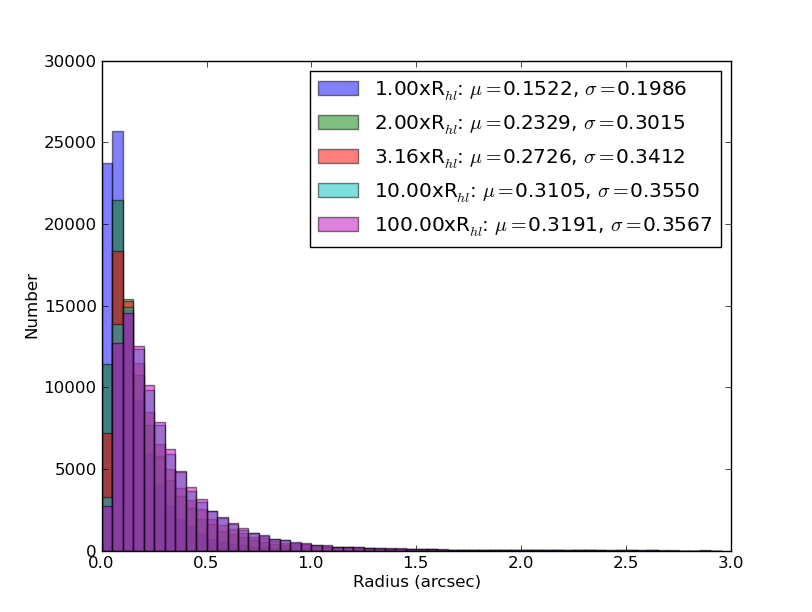
\includegraphics[width=5in]{validation_figures/half_light_hist.png}
\caption{\label{fig:hl_hist}}
\end{figure}
\begin{figure}[H]
\centering
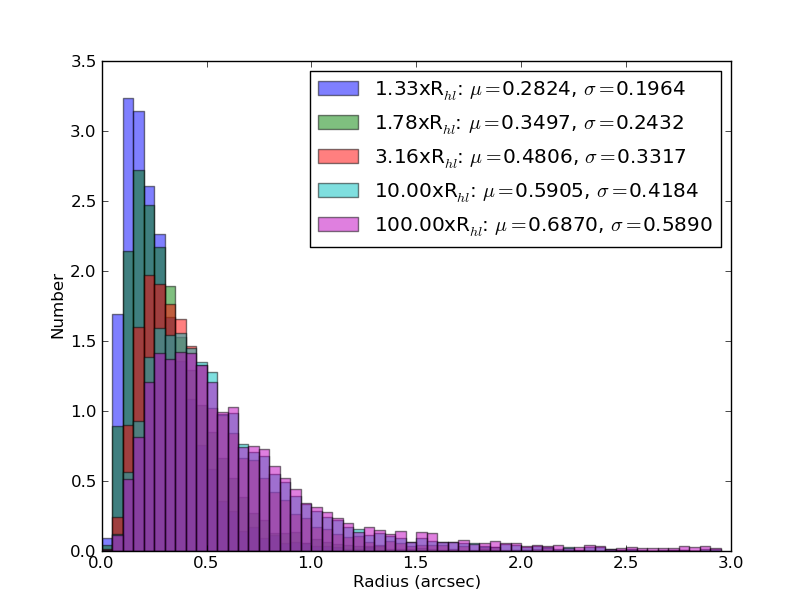
\includegraphics[width=5in]{validation_figures/Second_moment_hist.png}
\caption{\label{fig:mom_hist}}
\end{figure}
\begin{figure}[H]
\centering
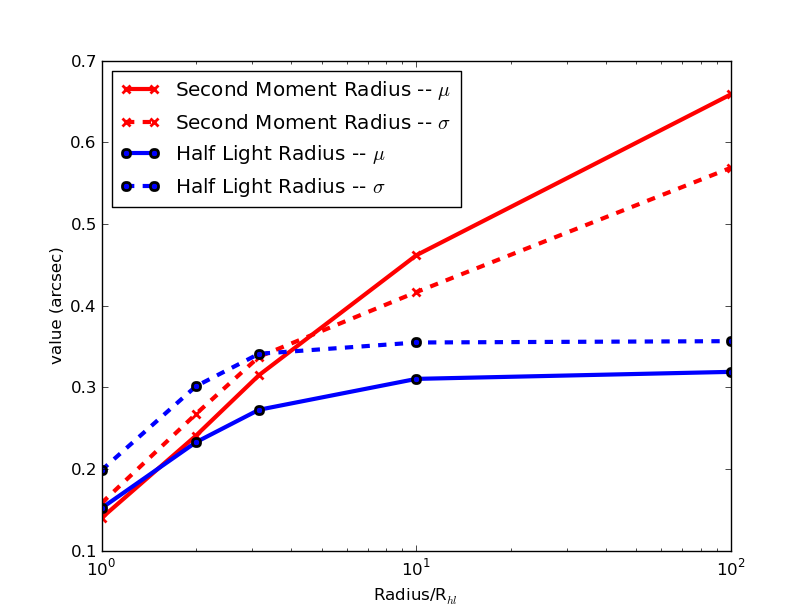
\includegraphics[width=5in]{validation_figures/sec_mom_half_light_mean_sigma.png}
\caption{\label{fig:mom_hl_line}}
\end{figure}

To test the sensitivity of $n_eff$ on the input half light radius distribution, we model the the half light distribution as a log normal distribution (see Figure
\ref{fig:hl_dist}).  Assuming that half light distribution is driven by the disk components, we choose the bulge distribution from the base catalog and then
choose a lognormal distribution with varying shape parameters to probe the size distribution space.
\begin{figure}[H]
\centering
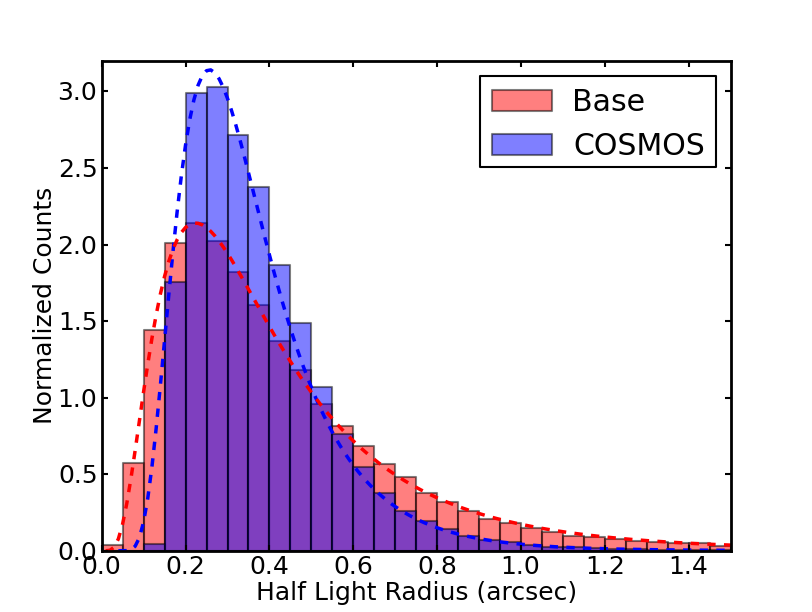
\includegraphics[width=5in]{validation_figures/ln_fit.png}
\caption{{\bf XXX This figure needs to be remade, it was done with only objects 20 - 24.5.}\label{fig:hl_dist}}
\end{figure}

Figure \ref{fig:size_sens} shows the sensitivity to the size distribution.  The x axis is related to the width of the 
distribution and the y axis is related to the location of the peak of the distribution. Over-plotted are points corresponding
to the best fit log normal distributions to the COSMOS data set and the base catalog data set.  The figure has been
normalized to the COSMOS distribution as truth.  This shows that the difference between the COSMOS distribution and
the base catalog distribution makes a difference less than 2.  This is well within the $\pm6$ stated by the requirements.
\begin{figure}[H]
\centering
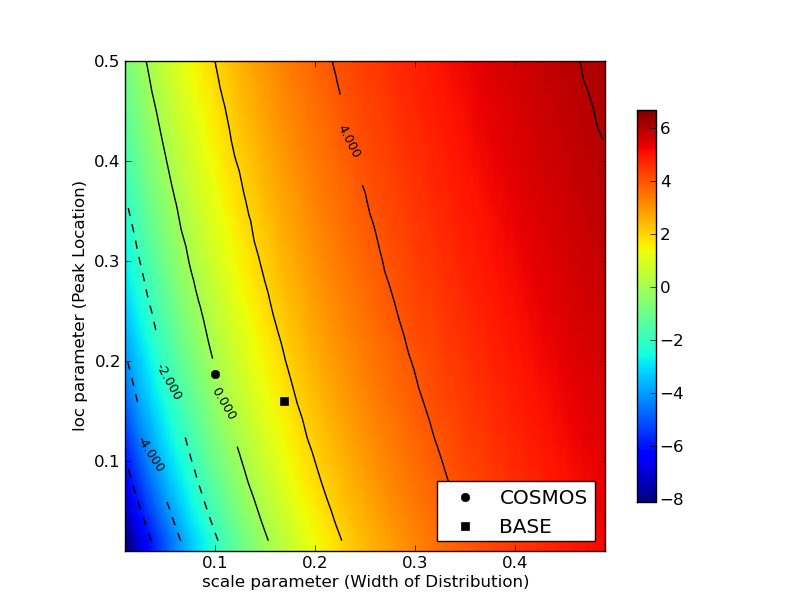
\includegraphics[width=5in]{validation_figures/size_sensitivity.png}
\caption{Sensitivity to the shape of the half light radius distribution.  The surface is normalized assuming the COSMOS distribution as truth.\label{fig:size_sens}}
\end{figure}


\subsection{Requirement 4: For the photometric calibration simulations
the distribution of stellar colors shall encompass the colors of white dwarfs through red giant branch stars.
The median color distributions of stars must trace the observed color locus for these stars to within 0.02 magnitudes
of the principal color (s,w,x,y) to the designed 5$\sigma$ single epoch limiting magnitude in the r-band.
{\bf update this for the most recent statement in the requirements document}}
For several reasons from calibration through to stellar populations work the Galactic model must have realistic color distributions.
This goes beyond simply spanning the proper color ranges.  The main sequence stellar locus must also agree with the location of the
stellar locus from other projects.  In Figure \ref{fig:starcolorspan} we show that the more trivial requirement that the stellar
colors span the ranges given in the requirements document is met.  Dashed lines in each panel show the requirements.  The measured
color distribution is plotted in the histogram.  The main sequence and red giant branch (RGB) contributions are plotted separately from
the white dwarf population.  Together the two distributions cover the required range.  The y-axis is log scale.
\begin{figure}[H]
\centering
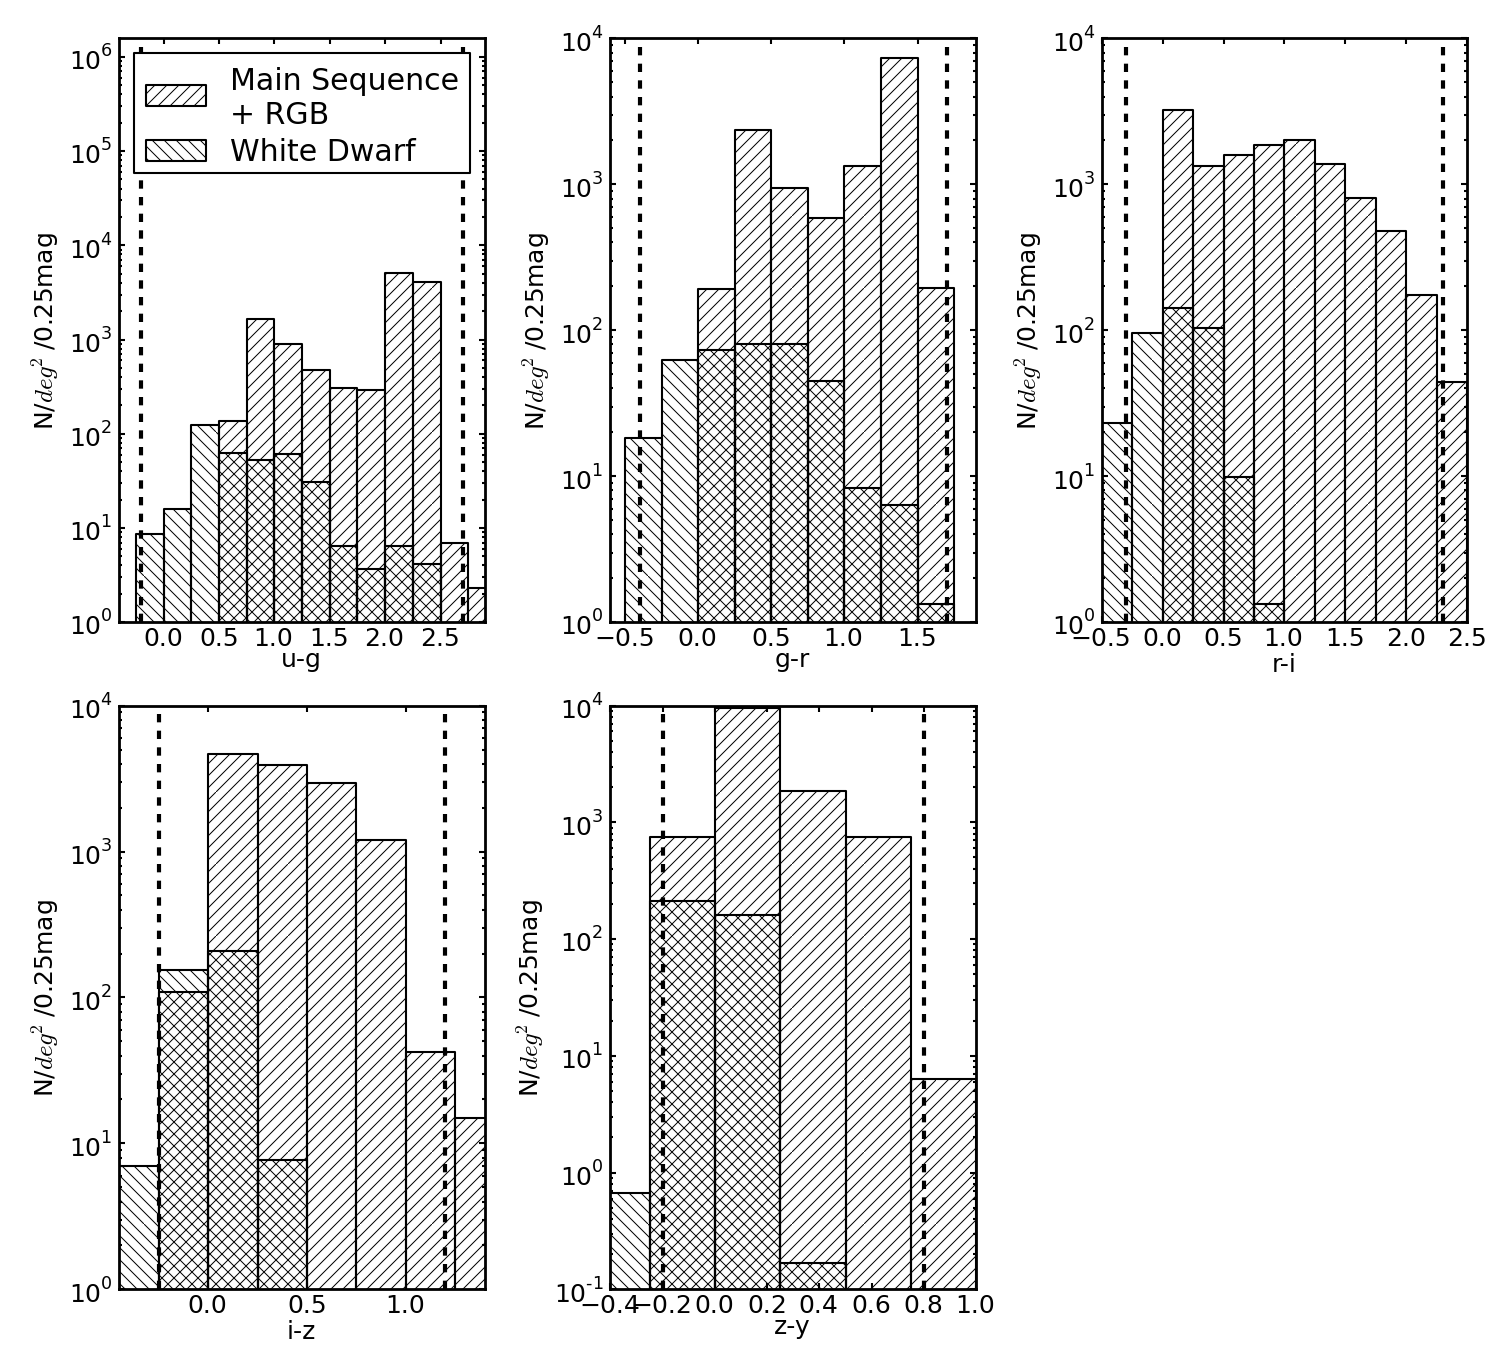
\includegraphics[width=5in]{validation_figures/star_lsst_color_hist.png}
\caption{Normalized counts of main sequence, red giant branch and white dwarf stars.  Heavy dashed lines show the requirements stated in the requirements document.\label{fig:starcolorspan}}
\end{figure}

To verify the veracity of the main sequence stellar locus, we use the principal colors of the stellar locus defined by \citet{helmi02} and 
fit for in the SDSS photometric \citet{ivezic04}.
We use stars selected from the same fields as used in the number counts analysis for all fields south of a galactic latitude of -30.
In order to avoid complications associated with the difference between the LSST and SDSS photometric systems, we calculate the un-extincted 
magnitudes in the SDSS bandpasses using the best fit spectrum for each star.  We then calculate
the principal colors for each star using the relations in \citet{ivezic04}, but removing the r-band dependence in $P\prime_{2}$.  Figure
\ref{fig:principalcolors} shows that the principal colors as calculated from the base catalog are in very good agreement with
the location of the stellar locus in the SDSS (zero color).  The base catalog easily meets the requirement of $\pm0.02mag$ deviation
from the stellar locus to single epoch depth in all 4 principal colors.  The scatter and trend with magnitude in the s color is due to 
the sensitivity of u-band on $[$Fe$/$H$]$.  Figure \ref{fig:sfeh} shows this dependence.  The transition from high metalicity disk stars to low 
metalicity halo stars introduces the scatter and slope.
\begin{figure}[H]
\centering
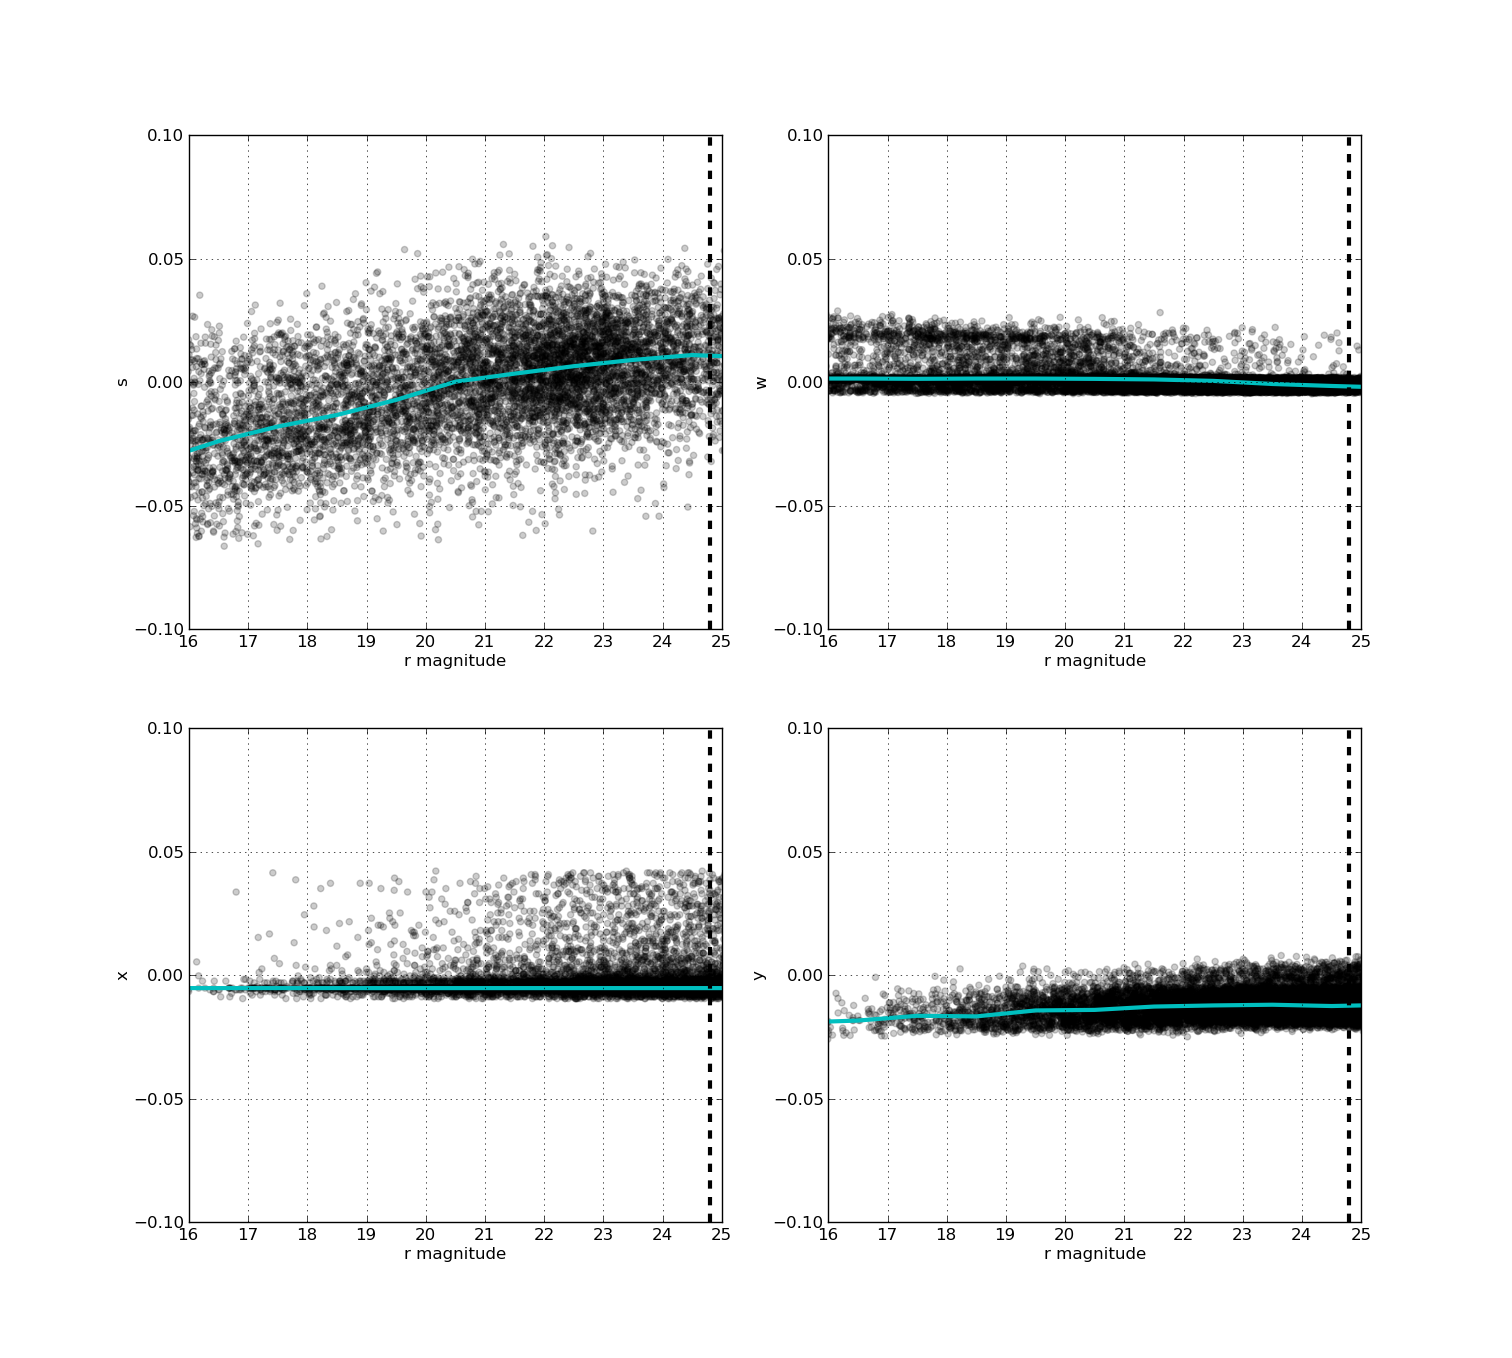
\includegraphics[width=5in]{validation_figures/principal_colors_vr.png}
\caption{Principal colors for the base catalog compared to the location of the stellar locus in the SDSS.\label{fig:principalcolors}}
\end{figure}

\begin{figure}[H]
\centering
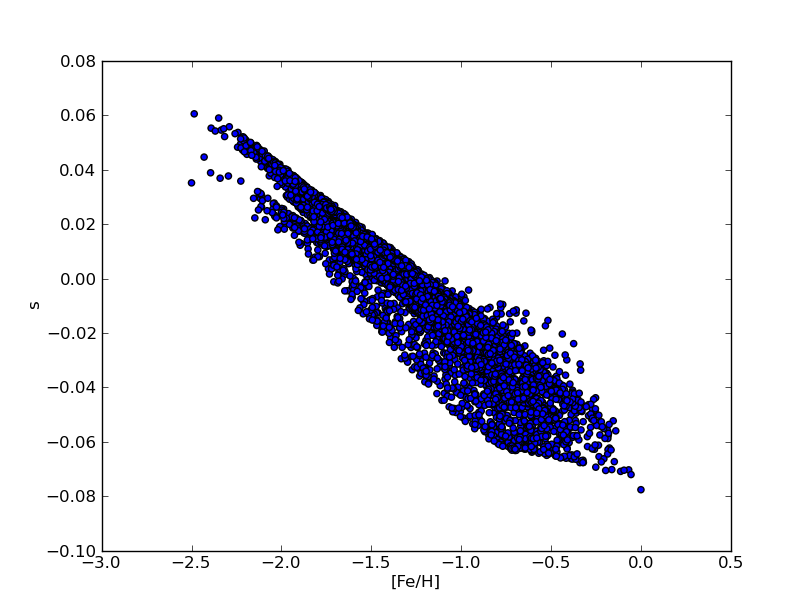
\includegraphics[width=5in]{validation_figures/s_met.png}
\caption{The principal color 's' as a function of metalicity.\label{fig:sfeh}}
\end{figure}


Figure \ref{fig:principalcolorshist} shows that the requirement of mean deviation from the color locus defined by the four principal colors by less than 
0.02 magnitudes is met in all four bands.
\begin{figure}[H]
\centering
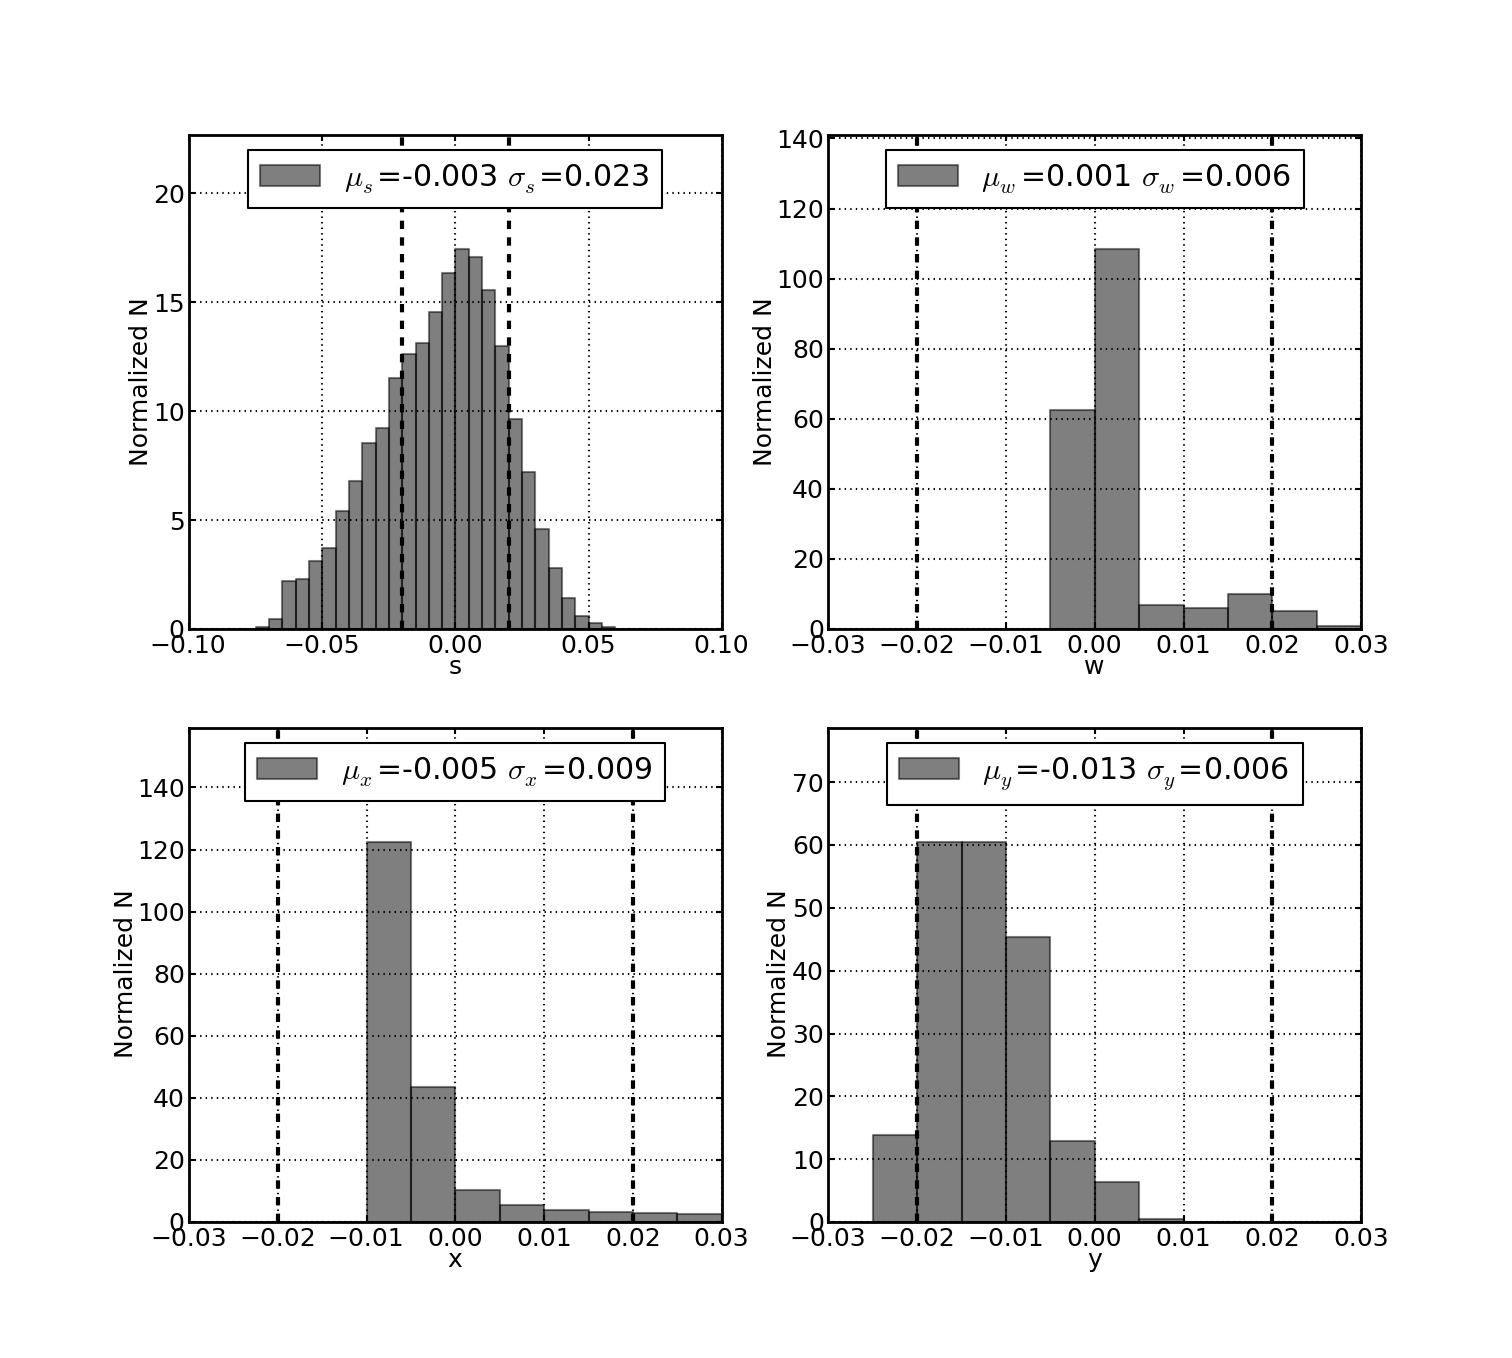
\includegraphics[width=5in]{validation_figures/principal_colors_hist.png}
\caption{Hisograms of the principal colors of stars in the base catalog to the stretch depth of r < 24.8. The mean and standard deviation for each 
histogram are given in the legend in the upper right.\label{fig:principalcolorshist}}
\end{figure}

\subsection{Requirement 5: All models for the astrometric transforms applied tothe catalogs (including interpolation functions) 
shall have an accuracy better than 1.6 mas}
All operations on positions are undertaken using double precision accuracy. Angular operations are converted to cartesian coordinates to provide accuracy at the celestial poles and to minimize the complications of the coordinate wraparound at the meridian. Astrometric accuracy of the CatSim simulation framework is determined from the performance of the Starlink positional astronomy library (SLALIB; \citet{wallace}). This software library enables astrometric transformations and operations with
accuracies on the order of a milliarcsecond or better.  The principal SLALIB routines used by the CatSim framework are those for precession, nutation, stellar aberration, rotation of the Earth, diurnal aberration, and refraction.  As described in \citet{wallace} the definition of ICRS coordinate system used in SLALIB and its transform to an FK5 (Fifth Fundamental Catalog - The Basic Fundamental Stars) system has an rms accuracy that is sub-milliarcsecond. Precession and nutation are based on the
model of \citet{SF2001} and have an rms uncertainty of $<$1 milliarcsecond (with the uncertainty growing at approximately 0.3 milliarcseconds per 1000 years). Aberration and light deflection corrections are undertaken in an iterative manner with uncertainties of $<$1 milliarcsecond and Earth position and velocity corrections are based on the methods of \citep{stumpff} with a maximum error of 0.3 milliarcseconds. All of these components, added in quadrature, meet the requirements described
in the simulation requirements document \citet{requirements}.

The largest of the uncertainties in any of the astrometric transforms is that due to the color dependence of refraction. For a nominal set of atmospheric conditions (i.e.\ temperature, pressure, humidity, and lapse rate) the rms uncertainty from 0.3 to 1 $\mu$m is 2.5 milliarcseconds. While refraction can be applied for science catalogs, for the catalogs generated as input to the LSST photon simulator refraction is not applied to the positions (i.e.\ it is generated internally to the photon
simulator).
\subsection{Requirement 6: The system shall be capable of incorporating new astrophysical catalogs without requiring
a redesign of the class-schema framework}
The ability to create new catalogs is available within the framework by the creation of user-designed subclasses and class mixins. A new type of catalog can be generated as a new class using the InstanceCatalog base class and other user-designed catalog classes (also using the InstanceCatalog base class) and class mixins. The columns desired in the new catalog are defined as class attributes. The data for these columns is gathered from the database directly or using methods defined in the class
for the catalog itself, in class mixins designed by the user, or in the base classes. These data gathering methods can take the form of a "get\_'column\_name'" method or in the form of compound columns with their own "get\_" methods. The required database column is then referred to in the "column\_by\_name()" method which returns the column values from the database. For example, the CustomCatalog below uses various aspects of this framework to write a new catalog to file:

\begin{verbatim}
class BasicCatalog(InstanceCatalog):
    """Simple catalog with columns directly from the database"""
    catalog_type = 'basic_catalog'
    refIdCol = 'id'
    column_outputs = ['id', 'ra_J2000', 'dec_J2000']
    # transformations specify conversions when moving from the database
    # to the catalog.  In this case, we take RA/DEC in radians and convert
    # to degrees.
    transformations = {"ra_J2000":np.degrees,
                       "dec_J2000":np.degrees}

class AstrometryMixin(object):
    @compound('ra_corrected', 'dec_corrected')
    def get_points_corrected(self):
        ra_J2000 = self.column_by_name('ra_J2000')
        dec_J2000 = self.column_by_name('dec_J2000')
    # ... do the conversions: these are just standins
    ra_corrected = ra_J2000 + 0.001
    dec_corrected = dec_J2000 - 0.001
    return ra_corrected, dec_corrected

class CustomCatalog(BasicCatalog, AstrometryMixin):
    catalog_type = 'custom_catalog'
    refIdCol = 'id'
    column_outputs = ['id', 'redshift', 'points_corrected']
    transformations = {"ra_corrected":np.degrees,
                       "dec_corrected":np.degrees}

# Now to create a catalog, we connect to a database and call write_catalog
db = GalaxyObj()
catalog = CustomCatalog(db)
catalog.write_catalog("out.txt")

# out.txt has the following columns:
# id redshift ra_corrected dec_corrected
\end{verbatim}

The InstanceCatalog metaclass verifies that all new columns desired in the user-defined catalog have associated means of gathering the required data from the database. If no method exists nor is there an associated database entry for the column directly then an error is raised. Furthermore, the error is raised before data begins transfer from the database because the instantiation of the class initiates a dry run of the table output. After the dry run the necessary database columns are verified
against the actual columns in the database and if there is a discrepancy the error is raised. As a result, the user is protected from errors after the data is pulled from the database and since all the necessary columns are determined during the dry run only one single query of the database is required to pull all necessary data.
\section{Future work}
We expect the requirements of the project to continue to evolve.  Informed by interations with the Systems Engineering team and the Data Management team we have 
identified several areas in which future development will likely take place.  Below we itemize these likely areas of future work.
\begin{itemize}
\item Implement bright stars -- For guiding and wavefront sensing analysis
\item Implementation of extended and morphological images -- Multifit, supernova analysis, galaxy models
\item Reduction of SED data size using PCA -- Parallelization of catalogs generation
\item Add errors to catalogs -- Calibration simulations
\item Add SNe to the catalogs to the framework -- Supernova sensitivity analysis
\item Increase size (area) of galaxy catalogs including cosmological signatures -- Large scale structure
\item Add weak lensing to the catalogs -- Weak lensing
\item Add extended stellar sources, e.g. clusters -- Deblending
\item General variability model -- Alert producton and light curve characterization
\item Further validation of the Milky Way model at low galactic latitudes
\end{itemize}
\bibliographystyle{plainnat}
\bibliography{validation}
\end{document}
